% XeLatex编辑
\documentclass[10pt, a4paper]{article}

\usepackage{ucas_matrix}
\usepackage{amsmath}

\begin{document}

\ucascover

% --- 目录 ---
% 会自动生成带“目录”标题的目录页
\tableofcontents
\newpage

% --- 正文开始 ---

\section{矩阵与线性方程组}

矩阵方法是数据科学、人工智能、大数据、机器学习等领域的核心基础,更是众多技术学科不可或缺的数学工具。从数学本质来看,矩阵的引入最初是为解决线性方程组问题,如今已发展为兼具基础性与实用性的核心数学工具。它不仅包含转置、内积、外积、逆矩阵、广义逆矩阵等基本运算,还涵盖行列式、范数、迹、秩等重要标量函数。本章将系统介绍矩阵与线性方程组的核心知识,为后续章节深入探讨矩阵分析及各类应用筑牢基础。

\subsection{线性方程组}

$\text{设有 n 个未知数 }m\text{ 个方程的线性方程组}$
\[\begin{cases}a_{11}x_{1}+a_{12}x_{2}+\cdots+a_{1n}x_{n}=b_{1},\\a_{21}x_{1}+a_{22}x_{2}+\cdots+a_{2n}x_{n}=b_{2},\\\cdots\cdots\cdots\cdots\\a_{m1}x_{1}+a_{m2}x_{2}+\cdots+a_{mn}x_{n}=b_{m},&\end{cases} (1)\]
其中$a_{ij}$是第$i$个方程的第$j$个未知数的系数,$b_i$是第$i$个方程的常数项$,i=1,2,\cdots,m;$ $j=1,2,\cdots,n$,当常数项$b_{1},b_{2},\cdots,b_{m}$不全为零时,线性方程组(1)叫做$n$元非齐次线性方程组,当$b_1,b_2,\cdots,b_m$ 全为零时,(1)式成为
\[\begin{cases}a_{11}x_{1}+a_{12}x_{2}+\cdots+a_{1n}x_{n}=0,\\a_{21}x_{1}+a_{22}x_{2}+\cdots+a_{2n}x_{n}=0,\\\cdots\cdots\cdots\cdots\\a_{m1}x_{1}+a_{m2}x_{2}+\cdots+a_{mn}x_{n}=0,&\end{cases}(2)\]
叫做$n$元齐次线性方程组

$n$ 元线性方程组往往简称为线性方程组或方程组.

对于$n$元齐次线性方程组$(2),x_1=x_2=\cdots=x_n=0$一定是它的解,这个解叫做齐次线性方程组(2)的零解.如果一组不全为零的数是(2)的解,则它叫做齐次线性方程组(2)的非零解.齐次线性方程组(2)一定有零解,但不一定有非零解.

例如
$$(1)\begin{cases}x-y=0,\\x+y=2;&\end{cases}(2)\begin{cases}x-y=0,\\x+y=1,\\x+y=2;&\end{cases}(3)\begin{cases}x_1-x_2=0,\\2x_1-2x_2=0,\\3x_1-3x_2=0&\end{cases}$$

就是三个二元线性方程组,并且(3)是齐次方程组。

下面讨论这三个方程组的解.方程组$\textcircled{1}:$易知其有惟一解 $x=y=1;$方程组$\textcircled{2}:$显然不存在数$x$ 和 $y$ 使 $x+y=1$ 和 $x+y=2$ 同时成立,故方程组$\textcircled{2}$无解;方程组$\textcircled{3}:设s$ 为任一数, 那么 $x_1=x_2=s$ 是$\textcircled{3}$的解,从而方程组$\textcircled{3}$有无限多个解.

这样看来,对于线性方程组需要讨论以下问题:(1)它是否有解?(2)在有解时它的解是否惟一?(3)如果有多个解,如何求出它的所有解?

对于线性方程组(1),上述诸问题的答案完全取决于它的$mn$个系数$a_{ij}\left(i=1,2,\cdots,\right.$$m;j=1,2,\cdots,n$)和右端的常数项$b_1,b_2,\cdotp\cdotp\cdotp,b_m$所构成的$m$行$n+1$列的矩形数表

\[\begin{array}{cccc}a_{11}&a_{12}&\cdots&a_{1n}\\a_{21}&a_{22}&\cdots&a_{2n}\\\vdots&\vdots&&\vdots\\a_{m1}&a_{m2}&\cdots&a_{mn}\end{array}\begin{array}{c}b_1\\b_2\\\vdots\\b_m\end{array}\]

这里横排称为行,竖排称为列;而对于齐次线性方程组(2)的相应问题的答案也完全取决于它的$mn$个系数$a_ij$ $(i=1,2,\cdots,m;j=1,2,\cdots,n)$所构成的$m$行$n$列的矩形数表

\[\begin{array}{cccc}a_{11}&a_{12}&\cdots&a_{1n}\\a_{21}&a_{22}&\cdots&a_{2n}\\\vdots&\vdots&\vdots&\vdots\\a_{m1}&a_{m2}&\cdots&a_{mn}\end{array}\]

$\text{由此我们引人矩阵的概念}.$
\subsection{高斯消元法与矩阵}

关于线性方程组的求解,有十分悠久的历史,我国古代名著《九章算术》就记载了求解线性方程组的一般方法,理论上的表述因德国数学家卡尔·高斯\footnote{卡尔·弗里德里希·高斯( 1777-1855)被许多人认为是有史以来最伟大的数学家之一,他令人惊叹的职业生涯需要数卷来记录。他被同行尊称为“数学之王”。在高斯去世后,其中一位同行写道:“他的思维深人了数字、空间和自然的最深奥秘;他测量了星星的轨迹,地球的形态和力量;他内化了未来一个世纪数学科学的演变。”历史证明了这一说法的正确性。}( Carl Gauss) 而被称为现在一般称这种方法为高斯消元法,以表彰他广泛使用并推广了这一方法。由于这种消元技术是基础性的,我们开始研究这一主题时,首先学习如何应用这种方法来计算线性方程的解。在掌握了计算方面的内容后,我们将转向围绕线性系统的更为理论性的方面。

问题是要在可能的情况下,计算含\( n \)个未知量的\( m \)个线性代数方程组的公共解。

\[\begin{aligned}&a_{11}x_1+a_{12}x_2+\cdots+a_{1n}x_n=b_1,\\&a_{21}x_1+a_{22}x_2+\cdots+a_{2n}x_n=b_2,\\&a_{m1}x_1+a_{m2}x_2+\cdots+a_{mn}x_n=b_m,\end{aligned}\]

其中\( x_i \)是未知量,\( a_{ij} \)和\( b_i \)是已知常数。\( a_{ij} \)被称为方程组的\textbf{系数},\( b_i\)的集合被称为方程组的\textbf{右侧项}。对于任何这样的方程组,解的集合恰好有三种可能性。

\begin{bluebox}{解集合的三种可能性}
	\begin{itemize}[leftmargin=*, labelsep=0.5em, itemsep=0.5em, topsep=0.5em]
		\item[■] \textbf{唯一解}:存在一组且仅有一组 $x_{i}$ 的值,同时满足所有方程
		\item[■] \textbf{无解}:不存在一组 $x_{i}$ 的值,同时满足所有方程—解集为空
		\item[■] \textbf{无限多解}:存在无穷多组不同的 $x_{i}$ 值,同时满足所有方程。很容易证明,如果一个系统有多个解,那么它就有无穷多个解。例如,一个系统不可能有确切的两个不同的解。
	\end{itemize}
\end{bluebox}

处理线性方程组的一部分工作是确定这三种可能性中哪一种成立。另一部分任务是,如果解唯一,则计算该解;如果有多个解,则描述所有解的集合。

高斯消元法是一种可用于实现所有这些目标的工具。高斯消元法是一种有条理的过程,通过依次消去未知量,将一个方程组系统地转化为另一个更简单但等价的方程组(如果两个方程组具有相同的解集,则称为\textbf{等价}的),最终得到一个易于求解的方程组。消元过程依赖于三种简单的运算,通过这些运算可以将一个方程组转化为另一个等价的方程组。为了描述这些运算,令\( E_k \)表示第\( k \)个方程。
\[E_k:a_{k1}x_1+a_{k2}x_2+\cdots+a_{kn}x_n=b_k\]

且将该方程组写为
\[\mathcal{S}=\begin{Bmatrix}E_{1}\\E_{2}\\\vdots\\E_{m}\end{Bmatrix}.\]

对于线性方程组\( \mathcal{S} \),以下三种\textbf{初等运算}中的每一种都会得到一个等价的方程组\( \mathcal{S}' \)。

\textbf{(1)} 交换第\( i \)个和第\( j \)个方程。即,若
\[\mathcal{S}=\begin{Bmatrix}E_{1}\\\vdots\\E_{i}\\\vdots\\E_{j}\\\vdots\\E_{m}\end{Bmatrix}, \mathrm{then} \mathcal{S}^{\prime}=\begin{Bmatrix}E_{1}\\\vdots\\E_{j}\\\vdots\\E_{i}\\\vdots\\E_{m}\end{Bmatrix}. (1.2.1)\]

\textbf{(2)} 用自身的一个非零倍数替换第\( i \)个方程。即,
\[\left.\mathcal{S}^{\prime}=\left\{\begin{array}{c}E_1\\\vdots\\\alpha E_i\\\vdots\\E_m\end{array}\right.\right\}, \mathrm{where} \alpha\neq0. (1.2.2)\]

\textbf{(3)} 用自身与第\( i \)个方程的一个倍数之和来替换第\( j \)个方程。即,
\[\left.S^{\prime}=\left\{\begin{array}{c}E_1\\\vdots\\E_i\\\vdots\\E_j+\alpha E_i\\\vdots\\E_m\end{array}\right.\right\}.(1.2.3)\]

为何这些运算都不会改变解集的解释留作练习。

实际中最常见的问题是具有\( n \)个方程和\( n \)个未知量的情况——称为\(\textbf{方形方程组}\),其有唯一解。由于高斯消元法在这种情况下较为直接,我们从这里开始,之后再讨论其他可能性。接下来详细描述将高斯消元法应用于以下简单(但典型)的方形方程组的过程:

\[\begin{aligned}2x+y+z=1,\\6x+2y+z=-1,\\-2x+2y+z=7.\end{aligned} (1.2.4)\]

在每一步中,策略是聚焦于一个称为\(\textbf{主元位置}\)的位置,并使用三种初等运算消去该位置下方的所有项。主元位置上的系数称为\(\textbf{主元元素}\)(或简称为\(\textbf{主元}\)),而主元所在的方程被称为\(\textbf{主元方程}\)。仅允许非零数作为主元。如果主元位置上的系数为0,则将主元方程与主元方程下方的某个方程交换,以得到非零主元。(对于具有唯一解的方形方程组,这总是可行的。)除非为0,否则第一个方程的第一个系数被选作第一个主元。例如,下方方程组中带圈的\textcircled{2}是第一步的主元:

\[\begin{array}{rcrcrcr}\textcircled{2}x&+&y&+&z&=&1,\\6x&+&2y&+&z&=&-1,\\-2x&+&2y&+&z&=&7.\end{array}\]

\textbf{步骤1.} 消去第一个主元下方的所有项。
\begin{itemize}
	\item 用第二个方程减去第一个方程的三倍,得到等价方程组:
\end{itemize}

\[
\begin{cases}
	\textcircled{2}x + y + z = 1, \\
	\quad - y - 2z = -4 \quad (E_2 - 3E_1), \\
	-2x + 2y + z = 7.
\end{cases}
\]

\begin{itemize}
	\item 将第一个方程加到第三个方程上,得到等价方程组:
\end{itemize}
\[
\begin{cases}
	\textcircled{2}x + y + z = 1, \\
	\quad - y - 2z = -4, \\
	\quad\quad 3y + 2z = 8 \quad (E_3 + E_1).
\end{cases}
\]

\textbf{步骤2.} 选择一个新的主元。
\begin{itemize}
	\item 暂时,通过向下并向右移动来选择一个新的主元\footnote{在数值计算中,选择主元的策略通常比单纯使用右下侧的下一个系数要复杂一些。目前先使用右下侧策略,之后会讨论更实用的策略。}。 若该系数不为0,则它是下一个主元。否则,与该位置下方的某个方程交换,以便将一个非零数带入该主元位置。在我们的例子中,$-1$是如下标识的第二个主元:
\end{itemize}
\[
\begin{cases}
	2x + y + z = 1, \\
	\textcircled{-1}y - 2z = -4, \\
	3y + 2z = 8.
\end{cases}
\]

\textbf{步骤3.} 消去第二个主元下方的所有项。
\begin{itemize}
	\item 将第二个方程的三倍加到第三个方程上,得到等价方程组:
\end{itemize}
\[
\begin{cases}
	2x + y + z = 1, \\
	\textcircled{-1}y - 2z = -4, \\
	-4z = -4 \quad (E_3 + 3E_2).
\end{cases}
\tag{1.2.5}
\]

\begin{itemize}
	\item 一般来说,在每一步中,你向下并向右移动以选择下一个主元,然后消去主元下方的所有项,直到无法继续进行。在本例中,第三个主元是\(-4\),但由于第三个主元下方没有需要消去的项,该过程完成。
\end{itemize}

此时,我们称该方程组已被\(\textbf{三角化}\)。三角方程组可通过一种称为\(\textbf{回代}\)的简单方法轻松求解,即先解最后一个方程得到最后一个未知量的值,然后将其代回倒数第二个方程,进而求解倒数第二个未知量,依此类推,直到每个未知量都被确定。对于我们的例子,解\((1.2.5)\)中的最后一个方程可得

\[ z = 1. \]

将\( z = 1 \)代回\((1.2.5)\)中的第二个方程并确定

\[ y = 4 - 2z = 4 - 2(1) = 2. \]

最后,将\( z = 1 \)和\( y = 2 \)代回\((1.2.5)\)中的第一个方程,得到

\[ x = \frac{1}{2}(1 - y - z) = \frac{1}{2}(1 - 2 - 1) = -1, \]

这就完成了求解。

显然,在每一步中,我们没有必要写下诸如“\( x \)”“\( y \)”“\( z \)”和“\( = \)”之类的符号,因为我们仅在处理系数。如果舍弃这些符号,线性方程组就简化为一个矩形数阵,其中每一行代表一个方程。例如,\((1.2.4)\)中的方程组可简化为如下数阵:

\[\begin{pmatrix}2&1&1&&1\\6&2&1&&-1\\-2&2&1&&7\end{pmatrix}. \text{(这条竖线强调了原来等号出现的位置。)}\]

系数的数阵——竖线左侧的数——被称为该方程组的\(\boxed{\text{系数矩阵}}\)。整个数阵——由方程组右侧的数扩充得到的系数矩阵——被称为与该方程组相关的\(\boxed{\text{增广矩阵}}\)。若系数矩阵记为\(\mathbf{A}\),右侧(常数列)记为\(\mathbf{b}\),则与该方程组相关的增广矩阵记为\([\mathbf{A}|\mathbf{b}]\)。

形式上,\textbf{标量}(scalar)是实数或复数,\textbf{矩阵}(matrix)是标量的矩形数阵。通常的惯例是用\textbf{大写粗体字母}表示矩阵,用对应的\textbf{带两个下标的小写字母}表示矩阵中的单个元素。例如,

\[
\mathbf{A} = \begin{pmatrix}
	a_{11} & a_{12} & \cdots & a_{1n} \\
	a_{21} & a_{22} & \cdots & a_{2n} \\
	\vdots & \vdots & \ddots & \vdots \\
	a_{m1} & a_{m2} & \cdots & a_{mn}
\end{pmatrix}.
\]

矩阵中单个元素的第一个下标指明该元素所在的\(\boxed{\text{行}}\)(水平线),第二个下标指明该元素所在的\(\boxed{\text{列}}\)(垂直线)。例如,若

\[\mathbf{A}=\begin{pmatrix}2&1&3&4\\8&6&5&-9\\-3&8&3&7\end{pmatrix}, \mathrm{then} a_{11}=2,a_{12}=1,\ldots,a_{34}=7. (1.2.6)\]

给定矩阵\(\mathbf{A}\)的\(\boxed{\text{子矩阵}}\)(submatrix)是通过删除\(\mathbf{A}\)的任意行和列组合得到的数阵。例如,\(\mathbf{B} = \begin{pmatrix} 2 & 4 \\ -3 & 7 \end{pmatrix}\)是\((1.2.6)\)中矩阵\(\mathbf{A}\)的子矩阵,因为\(\mathbf{B}\)是删除\(\mathbf{A}\)的第二行以及第二、三列后得到的结果。

当矩阵\(\mathbf{A}\)恰好有\( m \)行和\( n \)列时,称其\(\boxed{\text{形状}}\)或\(\boxed{\text{规模}}\)为\( m \times n \)(读作“\( m \) 乘 \( n \)”)。例如,\((1.2.6)\)中的矩阵是一个\( 3 \times 4 \)矩阵。按照约定,\( 1 \times 1 \)矩阵与标量视为同一对象,反之亦然。为了强调矩阵\(\mathbf{A}\)的形状是\( m \times n \),有时会给\(\mathbf{A}\)添加下标记为\(\mathbf{A}_{m \times n}\)。当\( m = n \)时(即\(\mathbf{A}\)的行数与列数相同),\(\mathbf{A}\)称为\(\boxed{\text{方阵}}\);否则,\(\mathbf{A}\)称为\(\boxed{\text{矩形矩阵}}\)。仅由一行或一列组成的矩阵通常分别称为\(\boxed{\text{行向量}}\)或\(\boxed{\text{列向量}}\)。

符号\(\mathbf{A}_{i*}\)用于表示第\( i \)行,而\(\mathbf{A}_{*j}\)表示矩阵\(\mathbf{A}\)的第\( j \)列。例如,若\(\mathbf{A}\)是\((1.2.6)\)中的矩阵,则

\[\mathbf{A}_{2*}=\begin{pmatrix}8&6&5&-9\end{pmatrix} \mathrm{and} \mathbf{A}_{*2}=\begin{pmatrix}1\\6\\8\end{pmatrix}.\]

对于一个线性方程组

\[\begin{aligned}&a_{11}x_1+a_{12}x_2+\cdots+a_{1n}x_n=b_1,\\&a_{21}x_1+a_{22}x_2+\cdots+a_{2n}x_n=b_2,\\&a_{m1}x_1+a_{m2}x_2+\cdots+a_{mn}x_n=b_m,\end{aligned}\]

高斯消元法可通过对相关增广矩阵\([\mathbf{A}|\mathbf{b}]\)的行执行**初等行变换**来实施,这些行变换对应于处理线性方程组时所用的三种初等运算\((1.2.1)\)、\((1.2.2)\)和\((1.2.3)\)。对于一个\( m \times n \)矩阵

\[\mathbf{M}=\begin{pmatrix}\mathbf{M}_{1*}\\\vdots\\\mathbf{M}_{i*}\\\vdots\\\mathbf{M}_{j*}\\\vdots\\\mathbf{M}_{m*}\end{pmatrix},\]

对矩阵\(\mathbf{M}\)的三种\(\boxed{\text{初等行变换}}\)(elementary row operations)类型如下。

- 类型I:交换第\( i \)行和第\( j \)行,得到
\[
\begin{pmatrix}
	\mathbf{M}_{1*} \\
	\vdots \\
	\mathbf{M}_{j*} \\
	\vdots \\
	\mathbf{M}_{i*} \\
	\vdots \\
	\mathbf{M}_{m*}
\end{pmatrix}
\tag{1.2.7}
\]

- 类型II:用自身的一个非零倍数替换第\( i \)行,得到
\[
\begin{pmatrix}
	\mathbf{M}_{1*} \\
	\vdots \\
	\alpha\mathbf{M}_{i*} \\
	\vdots \\
	\mathbf{M}_{m*}
\end{pmatrix}, \quad \text{where} \quad \alpha \neq 0.
\tag{1.2.8}
\]

- 类型III:用自身加上第\( i \)行的一个倍数的组合替换第\( j \)行,得到
\[
\begin{pmatrix}
	\mathbf{M}_{1*} \\
	\vdots \\
	\mathbf{M}_{i*} \\
	\vdots \\
	\mathbf{M}_{j*} + \alpha\mathbf{M}_{i*} \\
	\vdots \\
	\mathbf{M}_{m*}
\end{pmatrix}.
\tag{1.2.9}
\]

用初等行变换求解方程组(1.2.4)时,从相关的增广矩阵\( [\mathbf{A}|\mathbf{b}] \)开始,通过执行与对等式本身执行的初等运算完全对应的同一系列行变换,将系数矩阵\( \mathbf{A} \)三角化:
\[
\left(
\begin{array}{ccc|c}
	\boxed{2} & 1 & 1 & 1 \\
	6 & 2 & 1 & -1 \\
	-2 & 2 & 1 & 7 \\
\end{array}
\right)
\xrightarrow[R_3 + R_1]{R_2 - 3R_1}
\left(
\begin{array}{ccc|c}
	2 & 1 & 1 & 1 \\
	0 & \boxed{-1} & -2 & -4 \\
	0 & 3 & 2 & 8 \\
\end{array}
\right)
\xrightarrow{R_3 + 3R_2}
\left(
\begin{array}{ccc|c}
	2 & 1 & 1 & 1 \\
	0 & -1 & -2 & -4 \\
	0 & 0 & -4 & -4 \\
\end{array}
\right)
\]

最终的数阵表示三角方程组
\[\begin{aligned}2x+y+z=1,\\-y-2z=-4,\\-4z=-4\end{aligned}\]

它可以通过前面描述的回代法求解。一般来说,如果一个\( n \times n \)的方程组已被三角化为如下形式
\[
\begin{pmatrix}
	t_{11} & t_{12} & \cdots & t_{1n} & \big| & c_1 \\
	0 & t_{22} & \cdots & t_{2n} & \big| & c_2 \\
	\vdots & \vdots & \ddots & \vdots & \big| & \vdots \\
	0 & 0 & \cdots & t_{nn} & \big| & c_n \\
\end{pmatrix}
\tag{1.2.10}
\]

其中每个\( t_{ii} \neq 0 \)(即没有零主元),那么回代的一般算法如下。
\begin{bluebox}{回代算法}
	从(1.2.10)中确定\( x_i \)的值,首先令\( x_n = c_n / t_{nn} \),然后递归计算
	\[
	x_i = \frac{1}{t_{ii}} \left( c_i - t_{i,i+1}x_{i+1} - t_{i,i+2}x_{i+2} - \cdots - t_{in}x_n \right)
	\]
	其中\( i = n-1, n-2, \ldots, 2, 1 \)。
\end{bluebox}

评估算法效率的一种方法是统计所需的算术运算次数\footnote{仅靠运算次数来评估算法的效率,可能不再像过去那样重要了。老式计算机按顺序执行指令,而一些现代机器能够并行执行指令,因此不同的数值任务可以同时进行。适合并行化的算法可能运算次数更高,但在并行机器上的运行速度可能比运算次数较少但无法利用并行性的算法更快。仅靠运算次数来评估算法的效率,可能不再像过去那样重要了。老式计算机按顺序执行指令,而一些现代机器能够并行执行指令,因此不同的数值任务可以同时进行。适合并行化的算法可能运算次数更高,但在并行机器上的运行速度可能比运算次数较少但无法利用并行性的算法更快。}由于多种原因,加法和减法不做区分,乘法和除法也不做区分。此外,乘/除法通常与加/减法分开统计。即使你不深究细节,了解高斯消元法结合回代的运算次数也很重要,这样当遇到其他算法时,你就有了比较的依据。

\begin{bluebox}{高斯消元运算次数}
	对\( n \times n \)系统应用高斯消元结合回代,需要
	\[
	\frac{n^3}{3} + n^2 - \frac{n}{3} \quad \text{次乘/除法}
	\]
	和
	\[
	\frac{n^3}{3} + \frac{n^2}{2} - \frac{5n}{6} \quad \text{次加/减法}.
	\]
	当\( n \)增大时,\( n^3/3 \)项在这些表达式中占主导地位。因此,需要记住的重要点是,对\( n \times n \)系统进行高斯消元结合回代,大约需要\( n^3/3 \)次乘/除法,且加/减法的次数大致相同。
\end{bluebox}

% 红色文字
\textcolor{red}{例子1.2.1}
% 红色水平线(宽度为文本宽度,厚度0.4pt)
\color{red}\rule{\textwidth}{0.4pt}\color{black}

问题:用高斯消元结合回代法解下列方程组:
\[
\begin{cases}
	v - w = 3, \\
	-2u + 4v - w = 1, \\
	-2u + 5v - 4w = -2.
\end{cases}
\]

解:对应的增广矩阵为
\[
\begin{pmatrix}
	0 & 1 & -1 & \big| & 3 \\
	-2 & 4 & -1 & \big| & 1 \\
	-2 & 5 & -4 & \big| & -2
\end{pmatrix}.
\]

由于第一个主元位置是0,在消去第一个主元下方的元素之前,交换第一行和第二行:
\[
\begin{pmatrix}
	\boxed{0} & 1 & -1 & \big| & 3 \\
	-2 & 4 & -1 & \big| & 1 \\
	-2 & 5 & -4 & \big| & -2
\end{pmatrix}
\xrightarrow{\text{交换} R_1 \text{和} R_2}
\begin{pmatrix}
	\boxed{-2} & 4 & -1 & \big| & 1 \\
	0 & 1 & -1 & \big| & 3 \\
	-2 & 5 & -4 & \big| & -2
\end{pmatrix}
\xrightarrow{R_3 - R_1}
\begin{pmatrix}
	-2 & 4 & -1 & \big| & 1 \\
	0 & \boxed{1} & -1 & \big| & 3 \\
	0 & 1 & -3 & \big| & -3
\end{pmatrix}
\xrightarrow{R_3 - R_2}
\begin{pmatrix}
	-2 & 4 & -1 & \big| & 1 \\
	0 & 1 & -1 & \big| & 3 \\
	0 & 0 & -2 & \big| & -6
\end{pmatrix}
\]

回代得:

\[\begin{aligned}&w=\frac{-6}{-2}=3,\\&v=3+w=3+3=6,\\&u=\frac{1}{-2}\left(1-4v+w\right)=\frac{1}{-2}\left(1-24+3\right)=10.\end{aligned}\]

% 红色文字
\textcolor{red}{练习1.2}
% 红色水平线(宽度为文本宽度,厚度0.4pt)
\color{red}\rule{\textwidth}{0.4pt}\color{black}

\subsubsection{用高斯消元结合回代法解下列方程组:}
\[
\begin{cases}
	x_1 + x_2 + x_3 = 1, \\
	x_1 + 2x_2 + 2x_3 = 1, \\
	x_1 + 2x_2 + 3x_3 = 1.
\end{cases}
\]

\subsubsection{用高斯消元结合回代法解下列方程组:}
\[
\begin{cases}
	2x_1 - x_2 = 0, \\
	-x_1 + 2x_2 - x_3 = 0, \\
	-x_2 + x_3 = 1.
\end{cases}
\]
\subsubsection{用高斯消元结合回代法解下列方程组:}
\[
\begin{cases}
	4x_2 - 3x_3 = 3, \\
	-x_1 + 7x_2 - 5x_3 = 4, \\
	-x_1 + 8x_2 - 6x_3 = 5.
\end{cases}
\]

\subsubsection{解下列方程组:}
\[
\begin{cases}
	x_1 + x_2 + x_3 + x_4 = 1, \\
	x_1 + x_2 + 3x_3 + 3x_4 = 3, \\
	x_1 + x_2 + 2x_3 + 3x_4 = 3, \\
	x_1 + 3x_2 + 3x_3 + 3x_4 = 4.
\end{cases}
\]

\subsubsection{考虑以下三个系统,每个系统的系数相同,但右手边不同(这种情况经常出现):}
\[
\begin{cases}
	4x - 8y + 5z = 1 \big| 0 \big| 0, \\
	4x - 7y + 4z = 0 \big| 1 \big| 0, \\
	3x - 4y + 2z = 0 \big| 0 \big| 1.
\end{cases}
\]
通过对形式为\( [\mathbf{A} \mid \mathbf{b_1} \mid \mathbf{b_2} \mid \mathbf{b_3}] \)的增广矩阵执行高斯消元,一次性解出所有三个系统。

\subsubsection{假设矩阵\(\mathbf{B}\)是通过对矩阵\(\mathbf{A}\)执行一系列行变换得到的。解释为什么可以通过对\(\mathbf{B}\)执行行变换得到\(\mathbf{A}\)。}

\subsubsection{求满足以下条件的角\(\alpha\)、\(\beta\)和\(\gamma\):}
\[
\begin{cases}
	2\sin\alpha - \cos\beta + 3\tan\gamma = 3, \\
	4\sin\alpha + 2\cos\beta - 2\tan\gamma = 2, \\
	6\sin\alpha - 3\cos\beta + \tan\gamma = 9,
\end{cases}
\]
其中\(0 \leq \alpha \leq 2\pi\),\(0 \leq \beta \leq 2\pi\),且\(0 \leq \gamma < \pi\)。

\subsubsection{以下方程组无解:}
\[
\begin{cases}
	-x_1 + 3x_2 - 2x_3 = 1, \\
	-x_1 + 4x_2 - 3x_3 = 0, \\
	-x_1 + 5x_2 - 4x_3 = 0.
\end{cases}
\]
尝试用高斯消元法解这个方程组,并解释出现了什么情况表明该方程组无法求解。

\subsubsection{尝试用高斯消元法解方程组}
\[
\begin{cases}
	-x_1 + 3x_2 - 2x_3 = 4, \\
	-x_1 + 4x_2 - 3x_3 = 5, \\
	-x_1 + 5x_2 - 4x_3 = 6,
\end{cases}
\]
并解释为什么这个方程组一定有无穷多解。

\subsubsection{通过解一个\(3 \times 3\)方程组,求过点\((1,1)\)、\((2,2)\)和\((3,0)\)的抛物线\(y = \alpha + \beta x + \gamma x^2\)方程中的系数。}

\subsubsection{假设100只昆虫分布在一个由四个腔室组成的封闭空间中,腔室之间有如下所示的通道。}

\begin{figure}[h]
	\centering
	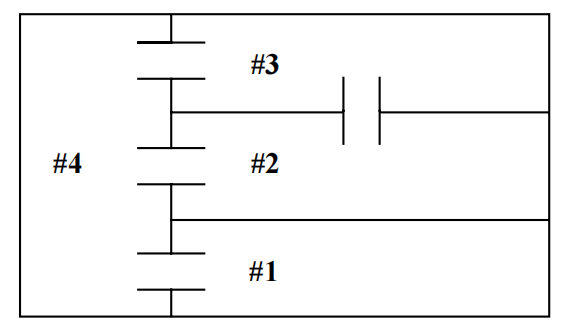
\includegraphics[width=\linewidth]{fig1.2.11} 
\end{figure}

一分钟后,昆虫重新分布。假设一分钟的时间不足以让一只昆虫访问超过一个腔室,且在一分钟结束时,每个腔室中40\%的昆虫没有离开它们在分钟开始时所处的腔室。离开一个腔室的昆虫会均匀分散到从其初始腔室可直接到达的腔室中——例如,从\#3出发,一半移向\#2,一半移向\#4。

(a) 若一分钟后,腔室\#1、\#2、\#3和\#4中分别有12、25、26和37只昆虫,确定初始分布必须是什么。

(b) 若初始分布是20、20、20、40,一分钟后的分布是什么?

\subsubsection{证明第8页讨论的三种初等行变换不独立,即通过(1.2.8)和(1.2.9)中的另外两种行变换序列可以完成交换操作(1.2.7)。}

\subsubsection{假设\([\mathbf{A}|\mathbf{b}]\)是线性系统的增广矩阵。你知道对\([\mathbf{A}|\mathbf{b}]\)执行行变换不会改变系统的解。然而,从未提及列操作,因为列操作会改变解。}
\begin{itemize}
	\item[(a)] 当列\(\mathbf{A}_{*j}\)和\(\mathbf{A}_{*k}\)交换时,描述对线性系统解的影响。
	\item[(b)] 当列\(\mathbf{A}_{*j}\)被\(\alpha\mathbf{A}_{*j}\)(\(\alpha \neq 0\))替换时,描述其影响。
	\item[(c)] 当列\(\mathbf{A}_{*j}\)被\(\mathbf{A}_{*j} + \alpha\mathbf{A}_{*k}\)替换时,描述其影响。
	提示:用2×2或3×3系统进行实验。
\end{itemize}

\subsubsection{考虑由下式定义的\(n \times n\)希尔伯特矩阵\(\mathbf{H}\):}
\[
\mathbf{H} = \begin{pmatrix}
	1 & \frac{1}{2} & \frac{1}{3} & \cdots & \frac{1}{n} \\
	\frac{1}{2} & \frac{1}{3} & \frac{1}{4} & \cdots & \frac{1}{n+1} \\
	\frac{1}{3} & \frac{1}{4} & \frac{1}{5} & \cdots & \frac{1}{n+2} \\
	\vdots & \vdots & \vdots & \cdots & \vdots \\
	\frac{1}{n} & \frac{1}{n+1} & \frac{1}{n+2} & \cdots & \frac{1}{2n-1}
\end{pmatrix}
\]
用\(i\)和\(j\)表示单个元素\(h_{ij}\)。

\subsubsection{验证文中给出的高斯消元结合回代法的运算次数对一般3×3系统是正确的。如果有挑战欲,尝试对一般\(n \times n\)系统验证这些次数。}

\subsubsection{解释为什么线性系统不可能恰好有两个不同的解。将你的论证扩展到解释:如果一个系统有多个解,那么它必须有无穷多个不同的解。}























\subsection{高斯-乔丹法}
本节的目的是介绍高斯消元法的一种变体,即\textbf{高斯-乔丹法}。
\footnote{尽管对于哪位Jordan应因该算法获得赞誉存在一些混淆,但现在看来很清楚,该方法实际上是由名为威廉·乔丹(WilhelmJordan,1842-1899)的大地测量学家提出的,而非更为人熟知的数学家玛丽·恩内蒙德·卡米尔·乔丹(Marie Ennemond Camille Jordan,1838-1922)。后者的名字常被错误地与该技术联系在一起,但他在矩阵分析的其他重要领域确实值得赞誉,其中最著名的是“乔丹标准型”。
	
威廉·乔丹出生于德国南部,在斯图加特接受教育,是卡尔斯鲁厄工学院的大地测量学教授。他是一位多产的作家,于1888年出版的《测量学手册》(Handbuch der Vermessungskunde)中介绍了他的消元方法。有趣的是,一种与W. 乔丹的高斯消元变体相似的方法,似乎被一位名叫克拉森(Clasen)的不知名法国人独立发现并描述。他似乎只发表过一篇科学文章,发表于1888年——与W. 乔丹的《手册》同年出版。}
高斯-乔丹法与标准高斯消元法的两个区别如下:

- 每一步都将主元强制化为1。

- 每一步都消去主元上方和下方的所有项。

换句话说,若线性系统的增广矩阵为
\[
\begin{pmatrix}
	a_{11} & a_{12} & \cdots & a_{1n} & \big| & b_1 \\
	a_{21} & a_{22} & \cdots & a_{2n} & \big| & b_2 \\
	\vdots & \vdots & \ddots & \vdots & \big| & \vdots \\
	a_{n1} & a_{n2} & \cdots & a_{nn} & \big| & b_n
\end{pmatrix}
\]
则通过初等行变换将其约化为
\[
\begin{pmatrix}
	1 & 0 & \cdots & 0 & \big| & s_1 \\
	0 & 1 & \cdots & 0 & \big| & s_2 \\
	\vdots & \vdots & \ddots & \vdots & \big| & \vdots \\
	0 & 0 & \cdots & 1 & \big| & s_n
\end{pmatrix}.
\]

此时解直接出现在最后一列(即\( x_i = s_i \)),因此该过程无需执行回代。

% 红色文字
\textcolor{red}{例子1.3.1}
% 红色水平线(宽度为文本宽度,厚度0.4pt)
\color{red}\rule{\textwidth}{0.4pt}\color{black}

问题:用高斯-乔丹法解下列方程组:
\[
\begin{cases}
	2x_1 + 2x_2 + 6x_3 = 4, \\
	2x_1 + x_2 + 7x_3 = 6, \\
	-2x_1 - 6x_2 - 7x_3 = -1.
\end{cases}
\]

解:操作序列在括号中注明,主元用圆圈标出。

\[
\begin{pmatrix}
	\boxed{2} & 2 & 6 & \big| & 4 \\
	2 & 1 & 7 & \big| & 6 \\
	-2 & -6 & -7 & \big| & -1
\end{pmatrix}
\xrightarrow{R_1/2}
\begin{pmatrix}
	\boxed{1} & 1 & 3 & \big| & 2 \\
	2 & 1 & 7 & \big| & 6 \\
	-2 & -6 & -7 & \big| & -1
\end{pmatrix}
\xrightarrow{\substack{R_2 - 2R_1 \\ R_3 + 2R_1}}
\]

\[
\rightarrow
\begin{pmatrix}
	\boxed{1} & 1 & 3 & \big| & 2 \\
	0 & -1 & 1 & \big| & 2 \\
	0 & -4 & -1 & \big| & 3
\end{pmatrix}
\xrightarrow{(-R_2)}
\begin{pmatrix}
	1 & 1 & 3 & \big| & 2 \\
	0 & \boxed{1} & -1 & \big| & -2 \\
	0 & -4 & -1 & \big| & 3
\end{pmatrix}
\xrightarrow{\substack{R_1 - R_2 \\ R_3 + 4R_2}}
\]

\[
\rightarrow
\begin{pmatrix}
	1 & 0 & 4 & \big| & 4 \\
	0 & \boxed{1} & -1 & \big| & -2 \\
	0 & 0 & -5 & \big| & -5
\end{pmatrix}
\xrightarrow{-R_3/5}
\begin{pmatrix}
	1 & 0 & 4 & \big| & 4 \\
	0 & 1 & -1 & \big| & -2 \\
	0 & 0 & \boxed{1} & \big| & 1
\end{pmatrix}
\xrightarrow{\substack{R_1 - 4R_3 \\ R_2 + R_3}}
\]

\[
\rightarrow
\begin{pmatrix}
	1 & 0 & 0 & \big| & 0 \\
	0 & 1 & 0 & \big| & -1 \\
	0 & 0 & \boxed{1} & \big| & 1
\end{pmatrix}
\]

因此,解为 \(\begin{pmatrix} x_1 \\ x_2 \\ x_3 \end{pmatrix} = \begin{pmatrix} 0 \\ -1 \\ 1 \end{pmatrix}\)。

% 红色水平线(宽度为文本宽度,厚度0.4pt)
\color{red}\rule{\textwidth}{0.4pt}\color{black}


从表面上看,高斯-乔丹消元法(Gauss-Jordan)和高斯消元法配合回代(Gaussian elimination with back substitution)似乎差别不大,因为在高斯-乔丹消元中,消去主元上方的项看起来就相当于进行回代。但这种观点是不正确的。高斯-乔丹消元法所需的运算量比带回代的高斯消元法更多。

\begin{bluebox}{高斯-乔丹法运算次数}
	对于 \( n \times n \) 系统,高斯-乔丹过程需要
	\[
	\frac{n^3}{2} + \frac{n^2}{2} \quad \text{次乘法/除法}
	\]
	以及
	\[
	\frac{n^3}{2} - \frac{n}{2} \quad \text{次加法/减法}.
	\]
	换句话说,高斯-乔丹法需要大约 \( n^3/2 \) 次乘法/除法,且加法/减法的次数也大致相同。
\end{bluebox}

回顾上一节,带回代的高斯消元法仅需要大约 \( \frac{n^3}{3} \) 次乘法/除法,且加法/减法的次数也大致相同。将其与高斯-乔丹法所需的 \( \frac{n^3}{2} \) 量级进行比较,可见高斯-乔丹法的运算量比带回代的高斯消元法大约多50\%。对于教材中常见的小型系统(例如 \( n = 3 \)),这种比较看不出明显差异。然而,在实际应用中,遇到的系统可能非常大,此时高斯-乔丹法与带回代的高斯消元法之间的差异会很显著。例如,若 \( n = 100 \),则 \( \frac{n^3}{3} \) 约为333,333,而 \( \frac{n^3}{2} \) 为500,000,两者在乘法/除法和加法/减法的次数上都相差166,667次。

尽管高斯-乔丹法不建议用于求解实际应用中出现的线性系统,但它确实有一些理论优势。此外,除了求解线性系统的解之外,它在其他任务中也可能是一种有用的技术。我们在讨论矩阵求逆时会用到高斯-乔丹过程——这是引入高斯-乔丹法的主要原因。

% 红色文字
\textcolor{red}{练习1.3}
% 红色水平线(宽度为文本宽度,厚度0.4pt)
\color{red}\rule{\textwidth}{0.4pt}\color{black}

\subsubsection{用高斯-乔丹法解下列方程组:}
\[
\begin{cases}
	4x_2 - 3x_3 = 3, \\
	-x_1 + 7x_2 - 5x_3 = 4, \\
	-x_1 + 8x_2 - 6x_3 = 5.
\end{cases}
\]

\subsubsection{用高斯-乔丹法解下列方程组:}
\[
\begin{cases}
	x_1 + x_2 + x_3 + x_4 = 1, \\
	x_1 + 2x_2 + 2x_3 + 2x_4 = 0, \\
	x_1 + 2x_2 + 3x_3 + 3x_4 = 0, \\
	x_1 + 2x_2 + 3x_3 + 4x_4 = 0.
\end{cases}
\]

\subsubsection{用高斯-乔丹法同时解下列三个方程组:}
\[
\begin{cases}
	2x_1 - x_2 = 1 \big| 0 \big| 0, \\
	-x_1 + 2x_2 - x_3 = 0 \big| 1 \big| 0, \\
	-x_2 + x_3 = 0 \big| 0 \big| 1.
\end{cases}
\]

\subsubsection{验证文中给出的高斯-乔丹法的运算次数对一般3×3系统是正确的。如果有挑战欲,尝试对一般\( n \times n \)系统验证这些次数。}





\subsection{2.4 齐次系统(Homogeneous Systems)}

\(n\) 个未知数的 \(m\) 个线性方程组
\[
\begin{array}{c}
    a_{11}x_1 + a_{12}x_2 + ... + a_{1n}x_n = 0, \\
    a_{21}x_1 + a_{22}x_2 + ... + a_{2n}x_n = 0, \\
    \vdots \\
    a_{m1}x_1 + a_{m2}x_2 + ... + a_{mn}x_n = 0.
\end{array}
\]

如果方程式的右侧完全由0组成,则称其为\textbf{齐次系统}。如果方程式的右侧至少有一个非零数,则该系统称为\textbf{非齐次系统}。本节旨在探讨齐次系统的一些基本概念。

在处理齐次方程组时,一致性从来都不是问题,因为无论系数值如何,
零解 \(x_1 = x_2 = ... = x_n = 0\) 始终是唯一解。下文中,
将全零组成的解称为\textbf{平凡解}。唯一的问题是:“除了平凡解之外,还有其他解吗?
如果有,我们如何才能最好地描述它们?” 和之前一样,高斯消元法可以给出答案。

使用高斯消元法将齐次系统的增广矩阵 \([\mathbf{A|0}]\) 化简为行阶梯形时,右侧的零列不会被任何三种基本行运算改变。
也就是说,任何通过行运算从 \([\mathbf{A|0}]\) 导出的行阶梯形,也必然具有 \([\mathbf{E|0}]\) 的形式。这意味着最后一列的零只是
多余的负担,没有必要在每一步都带上去。只需将系数矩阵 \(\mathbf{A}\) 化简为行阶梯形 \(\mathbf{E}\),并记住在执行回代时,右侧
完全为零。通过一个典型的例子,可以更好地理解这个过程。

为了求解齐次系统的解
\[
\begin{array}{c}
    x_1 + 2x_2 + 2x_3 + 3x_4 = 0, \\
    2x_1 + 4x_2 + x_3 + 3x_4 = 0, \\
    3x_1 + 6x_2 + x_3 + 4x_4 = 0,
\end{array}
\]
将系数矩阵简化为行阶梯形式。
\[
\mathbf{A} = 
\left(\begin{array}{cccc}
1 & 2 & 2 & 3 \\
2 & 4 & 1 & 3 \\
3 & 6 & 1 & 4
\end{array}\right)\to
\left(\begin{array}{cccc}
1 & 2 & 2 & 3 \\
0 & 0 & -3 & -3 \\
0 & 0 & -5 & -5
\end{array}\right)\to
\left(\begin{array}{cccc}
1 & 2 & 2 & 3 \\
0 & 0 & -3 & -3 \\
0 & 0 & 0 & 0
\end{array}\right)
= \mathbf{E}.
\]
因此,原始齐次系统等价于以下简化齐次系统:
\[
\begin{aligned}
    x_1 + 2x_2 + 2x_3 + 3x_4 &= 0, \\
    -3x_3 - 3x_4 &= 0.
\end{aligned}
\]
由于这个简化系统中有四个未知数,但只有两个方程,因此不可能为每个未知数求出唯一的解。我们能做的最好的事情是,
选择两个“基本”未知数——我们称之为\textbf{基本变量},并用另外两个未知数来求解它们——这两个未知数的值必须
保持任意或“自由”,因此它们被称为\textbf{自由变量}。虽然选择一组基本变量有多种可能性,但惯例是始终求解与枢轴位置对应的未知数,
或者,等价地,与基本列对应的未知数。在这个例子中,枢轴(以及基本列)位于第一和第三位置,
因此策略是应用回代法,用自由变量 \(x_2\) 和 \(x_4\) 来求解简化系统中的基本变量 \(x_1\) 和 \(x_3\)。由第二个方程得出
\[
x_3 = -x_4.
\]
代入第一个方程可得
\[
\begin{aligned}
x_1 &= -2x_2 -2x_3 - 3x_4, \\
&= -2x_2 - 2(-x_4) - 3x_4, \\
&= -2x_2 - x_4.
\end{aligned}
\]
因此,原齐次系统的所有解都可以描述为
\[
\begin{aligned}
    &x_1 = -2x_2 - x_4 \\
    &x_2 \text{ 任意}, \\
    &x_3 = -x_4, \\
    &x_4 \text{ 任意}.
\end{aligned}
\]
由于自由变量 \(x_2\) 和 \(x_4\) 取值范围涵盖所有可能值,上述表达式描述了所有可能的解。例如,当 \(x_2\) 和 \(x_4\) 取值
\(x_2 = 1\) 且 \(x_4 = -2\) 时,则有特定解
\[
x_1 = 0, x_2 = 1, x_3 = 2, x_4 = -2
\]
将来不再像上述那样描述解集,而是更方便地通过以下方式表达解集: 
\[
\left(\begin{array}{c}
x_1\\
x_2\\
x_3\\
x_4
\end{array}\right)=
\left(\begin{array}{c}
-2x_2 - x_4\\
x_2\\
-x_4\\
x_4
\end{array}\right)=
x_2\left(\begin{array}{c}
-2\\
1\\
0\\
0
\end{array}\right)+
x_4\left(\begin{array}{c}
-1\\
0\\
-1\\
1
\end{array}\right)
\]
假设 \(x_2\) 和 \(x_4\) 是自由变量,其取值范围为所有可能的数字。这种表示被称为齐次系统的\textbf{通解}。
通解的表达式强调,每个解都是两个特解的某种组合
\[
\mathbf{h}_1 = 
\left(\begin{array}{c}
-2\\
1\\
0\\
0
\end{array}\right),  
\mathbf{h}_2 =
\left(\begin{array}{c}
-1\\
0\\
-1\\
1
\end{array}\right).
\]
\(\mathbf{h}_1\) 和 \(\mathbf{h}_2\) 显然都是解,因为 \(\mathbf{h}_1\) 是在自由变量取值 \(x_2 = 1\) 和 \(x_4 = 0\) 时生成的,而
解 \(\mathbf{h}_2\) 是在 \(x_2 = 0\) 和 \(x_4 = 1\) 时生成的。

现在考虑一个由 \(m\) 个线性方程组 \([\mathbf{A|0}]\) 组成的广义齐次方程组,
其中有 \(n\) 个未知数。如果系数矩阵的 rank(\(\mathbf{A}\)) = \(r\),那么
从前面的讨论中应该可以明显看出,恰好有 \(r\) 个
基本变量(对应于 \(\mathbf{A}\) 中基本列的位置),以及
恰好有 \(n - r\) 个自由变量(对应于 \(\mathbf{A}\) 中非基本列的位置)。
使用高斯消元法将 \(\mathbf{A}\) 化为行阶梯形,
然后使用回代法根据自由变量求解基本变量,
即可得到\textbf{通解},其形式为
\[
\mathrm{x} = x_{f_1}\mathbf{h}_1 + x_{f_2}\mathbf{h}_2 + ... + x_{f_{n-r}}\mathbf{h}_{n-r},
\]
其中 \(x_{f_1}, x_{f_2}, ..., x_{f_{n-r}}\) 为自由变量,\(\mathbf{h}_1, \mathbf{h}_2, ..., \mathbf{h}_{n-r}\) 为
\(n \times 1\) 列,表示系统的特定解。由于自由变量 \(x_{f_i}\) 涵盖所有可能值,因此通解会生成所有可能的解。

通解并不依赖于所用的行阶梯形式,因为无论使用哪种行阶梯形式,使用回代法求解基本变量,都会生成一组唯一的特解,
{\(\mathbf{h}_1, \mathbf{h}_2, ..., \mathbf{h}_{n-r}\)}。无需赘述,我们可以认为这是正确的,因为使用任何行阶梯形式求解基本变量,
其结果必然与将 \(\mathbf{A}\) 完全简化为 \(\mathbf{E_A}\),然后求解简化齐次系统的基本变量,所得结果完全相同。\(\mathbf{E_A}\) 的唯一性,保证了 \(\mathbf{h}_i\) 的唯一性。

例如,如果与第一个系统相关的系数矩阵 \(\mathbf{A}\) 通过高斯-乔丹方法完全简化为 \(\mathbf{E_A}\)
\[
\mathbf{A} = 
\left(\begin{array}{cccc}
    1 & 2 & 2 & 3 \\
    2 & 4 & 1 & 3 \\
    3 & 6 & 1 & 4 \\
\end{array}\right)\to
\left(\begin{array}{cccc}
    1 & 2 & 0 & 1 \\
    0 & 0 & 1 & 1 \\
    0 & 0 & 0 & 0 \\
\end{array}\right)= \mathbf{E_A}
\]
然后我们得到以下简化系统:
\[
\begin{aligned}
    x_1 + 2x_2 + x_4 &= 0, \\
    x_3 + x_4 &= 0.
\end{aligned}
\]
用 \(x_2\) 和 \(x_4\) 来求解基本变量 \(x_1\) 和 \(x_3\),得到的结果与当时的推导给出的结果完全相同,因此也得到了与后续的通解完全相同的结果。

由于避免了回代过程,你可能会发现使用高斯-约当法将 \(\mathbf{A}\) 完全简化为 \(\mathbf{E_A}\) 更为方便,
然后直接从 \(\mathbf{E_A}\) 中的元素构建通解。这种方法通常会在示例和练习中采用。

如前所述,所有齐次系统都是一致的,因为由全零组成的平凡解始终是唯一解。一个自然而然的问题是:“平凡解何时是唯一解?”
换句话说,我们想知道齐次系统何时具有唯一解。上述的形式使答案显而易见。只要至少有一个自由变量,那么从上述可以清楚地看出,
将存在无数个解。因此,当且仅当没有自由变量时,平凡解才是唯一解。
由于自由变量的数量为 \(n - r\),其中 \(r\) = rank(\(\mathbf{A}\)),因此前面的陈述可以重新表述为:当且仅当 rank(\(\mathbf{A}\)) = \(n\),齐次系统才具有唯一解——平凡解。

% 红色文字
\textcolor{red}{例子2.4.1}
% 红色水平线(宽度为文本宽度,厚度0.4pt)
\color{red}\rule{\textwidth}{0.4pt}\color{black}

齐次系统
\[
\begin{aligned} 
    x_1 + 2x_2 + 2x_3 = 0, \\
    2x_1 + 5x_2 + 7x_3 = 0, \\
    3x_1 + 6x_2 + 8x_3 = 0.
\end{aligned}
\]
只有平凡解因为
\[
\mathbf{A} = 
\left(\begin{array}{ccc}
    1 & 2 & 2 \\
    2 & 5 & 7 \\
    3 & 6 & 8 \\
\end{array}\right)\to
\left(\begin{array}{cccc}
    1 & 2 & 2 \\
    0 & 1 & 3 \\
    0 & 0 & 2 \\
\end{array}\right) = \mathbf{E}
\]
表明 rank(\(\mathbf{A}\)) = \(n\) = 3。事实上,从 \(\mathbf{E}\) 中也可以看出,在系统 \([\mathbf{E|0}]\) 中应用反向替换只会产生平凡解。

% 红色文字
\textcolor{red}{例子2.4.2}
% 红色水平线(宽度为文本宽度,厚度0.4pt)
\color{red}\rule{\textwidth}{0.4pt}\color{black}

\textbf{问题}: 解释为什么下列齐次系统有无穷多个解,并给出通解:
\[
\begin{aligned} 
    x_1 + 2x_2 + 2x_3 = 0, \\
    2x_1 + 5x_2 + 7x_3 = 0, \\
    3x_1 + 6x_2 + 6x_3 = 0.
\end{aligned}
\]
\textbf{解答}: 
\[
\mathbf{A} = 
\left(\begin{array}{ccc}
    1 & 2 & 2 \\
    2 & 5 & 7 \\
    3 & 6 & 6 \\
\end{array}\right)\to
\left(\begin{array}{cccc}
    1 & 2 & 2 \\
    0 & 1 & 3 \\
    0 & 0 & 0 \\
\end{array}\right) = \mathbf{E}
\]
表明 rank(\(\mathbf{A}\)) = 2 < \(n\) = 3。由于基本列位于位置1 和 2,\(x_1\) 和 \(x_2\) 是基本变量,而 \(x_3\) 是自由变量。使用
\([E|0]\) 的反向代入,用自由变量来求解基本变量,可得 \(x_2 = -3x_3\) 和 \(x_1 = -2x_2 - 2x_3 = 4x_3\),因此通解为
\[
\left(\begin{array}{c}
    x_1 \\
    x_2 \\
    x_3 \\
\end{array}\right) = x_3
\left(\begin{array}{c}
    4 \\
    -3 \\
    1 \\
\end{array}\right), \text{其中} x_3 \text{是自由变量}.
\]
也就是说,每个解都是一个特定解 \(\mathbf{h}_1 = \left(\begin{array}{c} 4 \\-3 \\1\end{array}\right)\) 的倍数

\begin{bluebox}{总结}
设 \(\mathbf{A}_{m \times n}\) 为 \(m\) 个齐次线性方程组的系数矩阵,其中 \(n\) 个未知数,并设 rank(\(\mathbf{A}\)) = \(r\)。
\begin{itemize}
    \item 与基本列的位置(即枢轴位置)相对应的未知数称为\textbf{基本变量},与非基本列的位置相对应的未知数称为\textbf{自由变量}。
    \item 恰好有 \(r\) 个基本变量和 \(n-r\) 个自由变量。
    \item 为了描述所有解,使用高斯消元法将 \(\mathbf{A}\) 化为行阶梯形式,然后使用回代法求解,以自由变量的形式表示基本变量。这样就得到了通解,其形式为
    \[
    \mathrm{x} = x_{f_1}\mathbf{h}_1 + x_{f_2}\mathbf{h}_2 + ... + x_{f_{n-r}}\mathbf{h}_{n-r},
    \]
    其中 \(x_{f_1}, x_{f_2}, ..., x_{f_{n-r}}\) 为自由变量,\(\mathbf{h}_1, \mathbf{h}_2, ..., \mathbf{h}_{n-r}\) 为 \(n \times 1\) 列,表示齐次方程组的特解。\(\mathbf{h}_i\) 与回代过程中使用的
    行阶梯形式无关。由于自由变量 \(x_{f_i}\) 涵盖所有可能值,因此通解会生成所有可能的解。
    \item 一个齐次系统拥有唯一解(平凡解),当且仅当 rank(\(\mathbf{A}\)) = \(n\) ——即当且仅当不存在自由变量。
\end{itemize}
\end{bluebox}


% 红色文字
\textcolor{red}{练习 2.4}
% 红色水平线(宽度为文本宽度,厚度0.4pt)
\color{red}\rule{\textwidth}{0.4pt}\color{black}

\begin{enumerate}[leftmargin=*, label=\bfseries 2.4.\arabic*]

\item Determine the general solution for each of the following homogeneous systems.

\begin{enumerate}[label=(\alph*)]
    \item \(\begin{array}{l}
    x_1 + 2x_2 + x_3 + 2x_4 = 0, \\
    2x_1 + 4x_2 + x_3 + 3x_4 = 0, \\
    3x_1 + 6x_2 + x_3 + 4x_4 = 0.
    \end{array}\)
    
    \item \(\begin{array}{l}
    2x + y + z = 0, \\
    4x + 2y + z = 0, \\
    6x + 3y + z = 0, \\
    8x + 4y + z = 0.
    \end{array}\)
    
    \item \(\begin{array}{l}
    x_1 + x_2 + 2x_3 = 0, \\
    3x_1 + 3x_3 + 3x_4 = 0, \\
    2x_1 + x_2 + 3x_3 + x_4 = 0. \\
    x_1 + 2x_2 + 3x_3 - x_4 = 0,
    \end{array}\)

    \item \(\begin{array}{l}
    2x + y + z = 0, \\
    4x + 2y + z = 0, \\
    6x + 3y + z = 0, \\
    8x + 5y + z = 0.
    \end{array}\)
\end{enumerate}

\item Among all solutions that satisfy the homogeneous system
\[
\begin{aligned}
x + 2y + z &= 0, \\
2x + 4y + z &= 0, \\
x + 2y - z &=0.
\end{aligned}
\]
determine those that also satisfy the nonlinear constraint \(y - xy = 2z\).

\item Consider a homogeneous system whose coefficient matrix is
\[
\mathbf{A} = \left(\begin{array}{ccccc}
    1 & 2 & 1 & 3 & 1 \\
    2 & 4 & -1 & 3 & 8 \\
    1 & 2 & 3 & 5 & 7 \\
    2 & 4 & 2 & 6 & 2 \\
    3 & 6 & 1 & 7 & -3
\end{array}\right).
\]
First transform \(\mathbf{A}\) to an unreduced row echelon form to determine the
general solution of the associated homogeneous system. Then reduce \(\mathbf{A}\)
to \(\mathbf{E_A}\), and show that the same general solution is produced.

\item If \(\mathbf{A}\) is the coefficient matrix for a homogeneous system consisting of four equations in eight unknowns and if there are five free variables, what is rank(\(\mathbf{A}\))?

\item Suppose that \(\mathbf{A}\) is the coefficient matrix for a homogeneous system of four equations in six unknowns and suppose that \(\mathbf{A}\) has at least one nonzero row.
\begin{enumerate}[label=(\alph*)]
    \item Determine the fewest number of free variables that are possible.
    \item Determine the maximum number of free variables that are possible.
\end{enumerate}

\item Explain why a homogeneous system of \(m\) equations in \(n\) unknowns where \(m < n\) must always possess an infinite number of solutions.

\item Construct a homogeneous system of three equations in four unknowns that has
\[
x_2\left(\begin{array}{c}
    -2 \\
    1 \\
    0 \\
    0
\end{array}\right)+
x_4\left(\begin{array}{c}
    -1 \\
    0 \\
    -1 \\
    1
\end{array}\right)
\]
as its general solution.

\item If \(\mathbf{c}_1\) and \(\mathbf{c}_2\) are columns that represent two particular solutions of the same homogeneous system, explain why the sum \(\mathbf{c}_1 + \mathbf{c}_2\) must also represent a solution of this system.

\end{enumerate}

\subsection{让高斯消元法work}

你已经了解了高斯消元法的基本思想,让我们将其应用到实际问题中。
对于用笔和纸张进行的计算,我们一般是让情况尽可能简单,比如避免分数的出现,
以尽量减少计算失误的可能性。但是,现实世界的大部分问题没有这么“友好”。涉及
线性系统的实际应用我们通常会用到计算机。计算机不会采用分数,而是使用浮点数。
使用浮点数会产生一种可以预测的舍入误差,我们需要先了解这种误差和它对求解线性系统的影响。

计算机用浮点数来逼近实数,表示形式如下:

\begin{bluebox}{浮点数}
    一个$t$位,基数为$\beta$的\textit{\textbf{浮点数}}具有如下形式:
    $$f = \pm .d_{1} d_{2} \cdots d_{t} \times \beta^{\epsilon} \ \text{with} \ d_{1} \neq 0$$
    其中,基数$\beta$,指数$\epsilon$都是整数,且$d_{i}$是介于$0$和$\beta - 1$之间的整数。对于计算机而言,
    $\beta=2$比较常用,在纸笔上进行运算,通常取$\beta=10$。$t$和$\epsilon$的值取决于实际的硬件和软件。
\end{bluebox}

浮点数的表示形式只是我们熟悉的科学计数法的变体,在本文例子中我们一般取$\beta=10$。对于任意给定的$t$,$\beta$和$\epsilon$,显然它们能够表示的
实数集合$F$是有限集合。用浮点数来逼近实数的方法不止一种,因此,我们采用如下舍入约定:

给定一个实数$x$,$fl(x)$表示将$x$舍入到最接近的浮点数。如果$x$正好位于两个浮点数的中间,则取绝对值更大的那个浮点数。
取$t$位精度近似,当$\beta=10$,我们观察$x=.d_1d_2\cdots d_td_{t+1} \times 10^{\epsilon}$的$d_{t+1}$位($d_1\neq0$),
然后可以得到:
$$fl(x) = \begin{cases} .d_1d_2\cdots d_t \times 10^\epsilon & \text{if } d_{t+1} < 5, \\ ([.d_1d_2\cdots d_t] + 10^{-t}) \times 10^\epsilon & \text{if } d_{t+1} \ge 5. \end{cases}$$
举个例子, 在取$2$位精度近似,以10位基数的情况下,
$$fl(3/80) = fl(.0375) = fl(.375 \times 10^{-1}) = .38 \times 10^{-1} = .038.$$
考虑$\eta = 21/2$ 和$\xi =11/2$, 显然:
$$fl(\eta + \xi) \neq fl(\eta) + fl(\xi) \text{ 且\ } fl(\eta \times \xi) \neq fl(\eta) \times fl(\xi)$$

此外,实数运算中的若干常用法则在浮点运算中并不成立,结合律就是一个显著的例子。这一点,连同其他原因,使得浮点计算的分析工作颇具难度。
这一特性还意味着,你在处理本书中的例题与习题时必须格外谨慎。原因如下:尽管大多数计算器和计算机可被设置为显示不同位数的数字,但它们在显示结果前,所有计算都基于一个固定的内部精度完成,且该精度无法更改。你的计算器的内部精度,通常高于本书例题与习题所要求的精度。

因此,每当你用计算器进行$t$位精度的计算时,都应按以下步骤操作:

\begin{enumerate}
    \item 手动将计算结果舍入到$t$位有效数字。
    \item 在进行下一步计算前,将舍入后的数字重新手动输入计算器。
\end{enumerate}
换言之,不要在计算器或计算机中 “串联” 执行多个运算步骤。

为了更加详细了解如何使用浮点运算执行高斯消元法,让我们比较一下使用精确运算和使用$3$位精度和以$10$为基数的运算来求解以下系统:

$$\begin{cases}
    47x + 28y = 19 \\
    89x + 53y = 36
\end{cases}$$

使用精确计算的高斯消元法时,将第一个方程乘以乘数$m = 89/47$,然后从第二个方程中减去结果,得到:
$$\left(\begin{array}{cc|c}
    47 & 28 & 19 \\
    0 & -1/47 & 1/47
\end{array}\right) $$

回代得到精确解为$x=1$和$y=-1$。
使用$3$位精度浮点数进行高斯消元法时,乘数为:
$$fl(m) = fl(89/47) = .189 \times 10^1 = 1.89$$
由于
$$fl(fl(m) \times fl(47)) = fl(1.89 \times 47) = .888 \times 10^2 = 88.8$$
$$fl(fl(m) \times fl(28)) = fl(1.89 \times 28) = .529 \times 10^2 = 52.9$$
$$fl(fl(m) \times fl(19)) = fl(1.89 \times 19) = .359 \times 10^2 = 35.9$$
$3$位精度的高斯消元法第一步如下:
$$
\left(\begin{array}{cc|c}
    47 & 28 & 19 \\
    fl(89-88.8) & fl(53-52.9) & fl(36-35.9)
\end{array}\right) =
$$
$$
\left(\begin{array}{cc|c}
    47 & 28 & 19 \\
    \circlednum{.2} & .1 & .1
\end{array}\right)
$$
目标是将方程组三角化——在标记的$(2,1)$位置产生一个零,但使用3位精度消元法无法实现这一点。除非将标记的$\circlednum{.2}$替换为$0$,否则无法执行回代。此后,我们约定:\textit{无论实际出现的浮点数是多少,只需在要消去的位置填入$0$}。例如,在上述示例中,甚至无需计算
$$fl(89 - fl(fl(m) \times fl(47))) = fl(89 - 88.8) = 0.2$$
因此,上述示例的3位高斯消元法结果为:

$$
\left(\begin{array}{cc|c} 
47 & 28 & 19 \\
0 & .1 & .1
\end{array}\right)
$$
再应用3位精度回代,得到解为:
$$y = fl(.1/.1) = 1$$
$$x = fl(\frac{19-28}{47})=fl(\frac{-9}{47})=-.191$$
精确解$(1, -1)$与3位精度解$(-0.191, 1)$之间的巨大差异,说明了在尝试用浮点数算术求解线性方程组时可能遇到的一些问题。有时使用更高的精度可能会有所帮助,但这并不总是可行的——所有设备都有自然限制,使得超过一定程度后,扩展精度算术变得不切实际。即使有可能提高精度,也可能无法带来太多好处,因为在许多情况下,精度的提高并不会使累积的舍入误差相应减少。对于任何特定的精度(例如$t$),都不难构造出线性方程组的示例,其计算出的$t$位解与上述3位精度示例中的解一样糟糕。

尽管舍入的影响几乎永远无法消除,但有一些简单的技术可以帮助最小化这些机器引起的误差。

\begin{bluebox}{部分主元法}
在每一步,搜索主元位置及其下方的所有位置,找到绝对值最大的系数。如有必要,执行相应的行交换,将这个最大系数带入主元位置。下面展示了典型情况下的第三步:
$$
\left(\begin{array}{cccccc|c} 
* & * & * & * & * & * & * \\
0 & * & * & * & * & * & * \\
0 & 0 & \circlednum{s} & * & * & * & * \\
0 & 0 & S & * & * & * & * \\
0 & 0 & S & * & * & * & *
\end{array}\right)
$$
搜索第三列中标记为“\textbf{S}”的位置,找到绝对值最大的系数;如有必要,交换行,将该系数带入标记的主元位置。简而言之,策略是通过仅使用行交换,在每一步最大化主元的绝对值。


\end{bluebox}
表面上看,部分主元法为何能产生影响可能并不明显。下面的示例不仅表明部分主元法确实能产生很大的差异,还说明了该策略有效的原因。

\begin{example}
\label{example1.5.1}
容易验证方程组:
$$
\begin{cases} 
-10^{-4}x + y = 1, \\
x + y = 2
\end{cases}
$$
的精确解为:
$$
x = \frac{1}{1.0001}, \quad y = \frac{1.0002}{1.0001}
$$
若使用3位精度但不使用部分主元法,结果为:
$$
\left(\begin{array}{cc|c} 
-10^{-4} & 1 & 1 \\
1 & 1 & 2
\end{array}\right) \xrightarrow{R_2 + 10^4 R_1} \left(\begin{array}{cc|c} 
-10^{-4} & 1 & 1 \\
0 & 10^4 & 10^4
\end{array}\right)
$$
因为:
\begin{equation}
fl(1+10^4)=fl(.10001 \times 10^5) = .100 \times 10^5=10^4 \label{equation1.5.1}
\end{equation}
\begin{equation}
fl(2+10^4)=fl(.10002 \times 10^5) = .100 \times 10^5=10^4 \label{equation1.5.2}    
\end{equation}
回代可得:
$$
x = 0 \text{\ 且\ } y = 1
$$
尽管计算出的$y$的解接近精确解中的$y$,但计算出的$x$的解与精确解中的$x$相差甚远——计算出的$x$的解显然没有达到预期的三位有效数字精度。若使用3位精度且采用部分主元法,结果为:
$$
\left(\begin{array}{cc|c} 
-10^{-4} & 1 & 1 \\
1 & 1 & 2
\end{array}\right) \xrightarrow{} \left(\begin{array}{cc|c} 
1 & 1 & 2 \\
-10^{-4} & 1 & 1
\end{array}\right) \xrightarrow{R_2 + 10^{-4} R_1} \left(\begin{array}{cc|c} 
1 & 1 & 2 \\
0 & 1 & 1
\end{array}\right)
$$
因为:
\begin{equation}
fl(1 + 10^{-4}) = fl(.10001 \times 10^1) = .100 \times 10^1 = 1 \label{equation1.5.3}
\end{equation}
\begin{equation}
fl(1 + 2 \times 10^{-4}) = fl(0.10002 \times 10^1) = .100 \times 10^1 = 1 \label{equation1.5.4}
\end{equation}
此次回代得到计算解$x=1$,$y=1$,这与精确解的接近程度符合合理预期——计算解与精确解在3位有效数字上一致。

为什么部分主元法会产生差异?答案在于比较式\ref{equation1.5.1}、\ref{equation1.5.2}与式\ref{equation1.5.3}、\ref{equation1.5.4}

不使用部分主元法时,乘数为$10^4$,这个数值太大,完全掩盖了相对较小的数字$1$和$2$的算术运算,导致它们无法被考虑在内。也就是说,较小的数字$1$和$2$被“淹没”了,仿佛从未存在过,因此$3$位精度计算得到的是另一个方程组的精确解,该方程组与原方程组差异很大:
$$
\left(\begin{array}{cc|c}
-10^{-4} & 1 & 1 \\
1 & 0 & 0
\end{array}
\right)    
$$
使用部分主元法时,乘数为$10^{-4}$,这个数值足够小,不会淹没数字$1$和$2$。在这种情况下,$3$位精度计算得到的是方程组$\left(\begin{array}{cc|c}0 & 1 & 1 \\ 1 & 1 & 2\end{array}\right)$的精确解,该方程组与原方程组接近。

\end{example}

总之,示例\ref{example1.5.1}中的“罪魁祸首”是较大的乘数,它导致一些较小的数字无法被充分考虑,从而得到与原方程组差异很大的另一个方程组的精确解。通过在每一步最大化主元的绝对值,我们最小化了相关乘数的绝对值,从而有助于控制消元过程中出现的数字的增长,进而有助于规避舍入误差的一些影响。

当使用部分主元法时,所有乘数的绝对值都不会超过1。要理解这一点,考虑消元过程中的以下两个典型步骤:
$$
\left(\begin{array}{cccccc|c} 
* & * & * & * & * & * & * \\
0 & * & * & * & * & * & * \\
0 & 0 & \circlednum{p} & * & * & * & * \\
0 & 0 & q & * & * & * & * \\
0 & 0 & r & * & * & * & *
\end{array}\right) \xrightarrow[R_4 - (q/p)R_3]{R_5 - (r/p)R_3}
\left(
    \begin{array}{cccccc|c}
        * & * & * & * & * & * & * \\
        0 & * & * & * & * & * & * \\
        0 & 0 & \circlednum{p} & * & * & * & * \\
        0 & 0 & 0 & * & * & * & * \\
        0 & 0 & 0 & * & * & * & *
    \end{array}
\right)
$$
主元为$p$,而$q/p$和$r/p$是乘数。若采用了部分主元法,则$|p| \geq |q|$且$|p| \geq |r|$,因此:
$$
\left|\frac{q}{p}\right| \leq 1, \quad \left|\frac{r}{p}\right| \leq 1
$$
通过确保所有乘数的绝对值不超过1,产生相对较大数字(可能淹没较小数字重要性)的可能性大大降低,但这并未完全消除。要看到仍有改进空间,考虑以下示例。

\begin{example}
\label{example1.5.2}
方程组:
$$
\begin{cases} 
-10x + 10^5y = 10^5, \\
x + y = 2
\end{cases}
$$
的精确解为:
$$
x = \frac{1}{1.0001}, \quad y = \frac{1.0002}{1.0001}
$$
假设使用3位精度且采用部分主元法。由于$|-10| > 1$,无需交换行,得到:
$$
\left(\begin{array}{cc|c} 
-10 & 10^5 & 10^5 \\
1 & 1 & 2
\end{array}\right) \xrightarrow{R_2 + 10^{-1} R_1} \left(\begin{array}{cc|c} 
-10 & 10^5 & 10^5 \\
0 & 10^4 & 10^4
\end{array}\right)
$$
\end{example}
回代得到解为:
$$x=0, \quad y=1$$
这个结果必须被认为是非常糟糕的——计算出的$y$的3位解还不错,但计算出的$x$的3位解非常差!

示例\ref{example1.5.2}中的问题根源是什么?此次不能归咎于乘数。问题在于第一个方程中的系数远大于第二个方程中的系数,即由于系数的数量级不同,存在尺度问题。因此,在尝试求解方程组之前,应该以某种方式对其进行尺度变换。

若将上述示例中的第一个方程进行尺度变换,确保绝对值最大的系数为1(通过将第一个方程乘以$10^{-5}$),则得到示例\ref{example1.5.2}中的方程组,我们知道通过部分主元法可以得到与精确解非常接近的近似解。

这表明部分主元法的成功可能取决于保持系数之间的适当尺度。因此,使高斯消元法实用的第二个改进是合理的尺度变换策略。不幸的是,目前还没有已知的尺度变换方法能对所有可能的方程组都产生最优结果,因此我们必须满足于一种在大多数情况下都能工作的策略。该策略是将行尺度变换(将选定的行乘以非零乘数)与列尺度变换(将系数矩阵$A$的选定列乘以非零乘数)相结合。

行尺度变换不会改变精确解,但列尺度变换会改变精确解。列尺度变换相当于改变第$k$个未知数的单位。例如,若增广矩阵$[A|b]$中第$k$个未知数$x_k$的单位是毫米,且将$A$的第$k$列乘以$0.001$,则尺度变换后的方程组$[\hat{A}|b]$中的第$k$个未知数为$\hat{x}_k = 1000x_k$,因此尺度变换后的未知数$\hat{x}_k$的单位变为米。

经验表明,以下结合行尺度变换和列尺度变换的策略通常能很好地工作:

\begin{bluebox}{实用尺度变换策略}
\begin{itemize}
    \item 选择与问题自然相关的单位,且不扭曲事物大小之间的关系。这些自然单位通常是显而易见的,在此之后通常不再尝试进一步的列尺度变换。
    \item 对增广矩阵$[A|b]$进行行尺度变换,使得$A$的每一行中绝对值最大的系数等于1。也就是说,将每个方程除以其绝对值最大的系数。
\end{itemize}
部分主元法与上述尺度变换策略相结合,使带回代的高斯消元法成为一种极其有效的工具。长期以来,这种技术已被证明能可靠地求解实际工作中遇到的大多数线性方程组。
\end{bluebox}
尽管应用不广泛,但存在一种部分主元法的扩展形式,称为完全主元法,在某些特殊情况下,它在帮助控制舍入误差的影响方面可能比部分主元法更有效。

\begin{bluebox}{完全主元法}
若$[A|b]$是高斯消元法第$k$步的增广矩阵,则搜索主元位置以及$A$中主元位置下方和右侧的所有位置,找到绝对值最大的系数。如有必要,执行相应的行交换和列交换,将绝对值最大的系数带入主元位置。下面展示了典型情况下的第三步:
$$
\left(\begin{array}{cccccc|c} 
* & * & * & * & * & * & * \\
0 & * & * & * & * & * & * \\
0 & 0 & \circlednum{s} & S & S & * & * \\
0 & 0 & S & S & S & * & *
\end{array}\right)
$$

搜索标记为“S”的位置,找到绝对值最大的系数;如有必要,交换行和列,将该最大系数带入标记的主元位置。$A$中列交换的效果相当于对相关未知数进行置换(或重命名)。
\end{bluebox}

不难看出,完全主元法至少应与部分主元法一样有效。此外,有可能构造出特殊示例,其中完全主元法优于部分主元法。然而,在实际应用中很少遇到此类方程组。

\begin{example}
\label{example1.5.3}
问题:使用3位精度和完全主元法求解以下方程组:
$$
\begin{cases} 
    x - y = -2, \\
-9x + 10y = 12
\end{cases}
$$
解:由于10是搜索范围内绝对值最大的系数,交换第一行和第二行,然后交换第一列和第二列:
$$
\left(\begin{array}{cc|c} 
1 & -1 & -2 \\
-9 & 10 & 12 
\end{array}\right) \xrightarrow{} \left(\begin{array}{cc|c} 
-9 & 10 & 12 \\
1 & -1 & -2 
\end{array}\right) \xrightarrow{} \left(\begin{array}{cc|c} 
10 & -9 & 12 \\
-1 & 1 & -2 
\end{array}\right) \xrightarrow{} \left(\begin{array}{cc|c}
10 & -9 & 12 \\
0 & 1 & -8    
\end{array}\right)
$$
列交换的效果是将未知数重命名为$\hat{x}$和$\hat{y}$,其中$\hat{x}=y$,$\hat{y}=x$。回代得到:
$$x=\hat{y}=-8, \quad y=\hat{x}=-6$$

在这种情况下,3位解与精确解一致。若仅使用部分主元法,3位解的精度不会这么高。但如果使用带尺度变换的部分主元法,结果与使用完全主元法的结果相同。
\end{example}

如果使用完全主元法的成本与使用部分主元法的成本几乎相同,我们会始终使用完全主元法。然而,不难证明,完全主元法的成本大约是直接高斯消元法的两倍,而部分主元法仅增加微不足道的成本。再加上在实际应用中,极少遇到带尺度变换的部分主元法不足以处理但完全主元法可以处理的方程组,因此很容易理解为什么完全主元法在实践中很少使用。对于中等规模的稠密方程组(即没有大量零元素的方程组),带尺度变换的部分主元法的高斯消元法是首选方法。

\begin{exercise}
考虑下面的方程组:
$$
\begin{cases} 
10^{-3}x - y = 1, \\
x + y = 0
\end{cases}
$$
\begin{enumerate}[label=(\alph*)]
    \item 使用3位精度且不使用主元法求解该方程组。\label{item1.5.1.a}
    \item 找到一个由\ref{item1.5.1.a}中解精确满足的方程组,并指出该方程组与原方程组的接近程度。
    \item 现在使用部分主元法和3位精度求解原方程组。\label{item1.5.1.b}
    \item 找到一个由\ref{item1.5.1.b}中解精确满足的方程组,并指出该方程组与原方程组的接近程度。
    \item 使用精确算术求解原方程组,并将精确解与\ref{item1.5.1.a}和\ref{item1.5.1.b}的结果进行比较。
    \item 将精确解舍入到三位有效数字,并与\ref{item1.5.1.a}和\ref{item1.5.1.b}的结果进行比较。
\end{enumerate}
\end{exercise}

\begin{exercise}
考虑以下方程组:
$$
\begin{cases} 
    x + y = 3, \\
 -10x + 10^5y = 10^5
\end{cases}
$$
\begin{enumerate}[label=(\alph*)]
    \item 使用4位算术、部分主元法且不进行尺度变换,计算方程组的解。\label{item1.5.2.a}
    \item 使用4位算术、完全主元法且不进行尺度变换,计算原方程组的解。\label{item1.5.2.b}
    \item 此次先对原方程组进行行尺度变换,然后使用4位算术和部分主元法计算方程组的解。\label{item1.5.2.c}
    \item 现在确定方程组的精确解,并将其与\ref{item1.5.2.a}、\ref{item1.5.2.b}和\ref{item1.5.2.c}的结果进行比较。
\end{enumerate}
\end{exercise}

\begin{exercise}
在不进行尺度变换的情况下,分别使用无部分主元法和部分主元法,计算以下方程组的3位解,将结果与精确解进行比较。
$$
\begin{cases} 
-3x + y = -2, \\
10x - 3y = 7
\end{cases}
$$
\end{exercise}

\begin{exercise}
考虑以下方程组,其系数矩阵为希尔伯特矩阵:
$$
\begin{cases} 
x + \frac{1}{2}y + \frac{1}{3}z = \frac{1}{3}, \\
\frac{1}{2}x + \frac{1}{3}y + \frac{1}{4}z = \frac{1}{3}, \\
\frac{1}{3}x + \frac{1}{4}y + \frac{1}{5}z = \frac{1}{3}
\end{cases}
$$
\begin{enumerate}[label=(\alph*)]
    \item 首先将系数转换为3位浮点数,然后使用3位算术、部分主元法但不进行尺度变换,计算方程组的解。\label{item1.5.4.a}
    \item 再次使用3位算术,但先将系数(转换为浮点数后)进行行尺度变换,然后使用部分主元法计算方程组的解。\label{item1.5.4.b}
    \item 按照(b)中的步骤进行,但此次在每一步消元前都对系数进行行尺度变换。\label{item1.5.4.c}
    \item 现在使用精确算术对原方程组求解,得到精确解,并将结果与\ref{item1.5.4.a}、\ref{item1.5.4.b}和\ref{item1.5.4.c}的结果进行比较。
\end{enumerate}
\end{exercise}

\subsection{不良系统}

在适当缩放的系统上进行部分旋转的高斯消除可能是线性代数实际应用中最基本的算法。但它不是通用算法,也不能盲目使用。本节的目的是指出,在求解线性系统时,必须始终谨慎行事,因为有些系统对小扰动非常敏感,以至于无法放心使用数值技术。

\begin{example}
\label{example1.6.1}
考虑方程组:
$$
\begin{cases} 
.835x + .667y = .168, \\
.333x + .266y = .067
\end{cases}
$$
其精确解为$x=1$,$y=-1$。
若仅将$b_2=.067$轻微扰动为$\hat{b}_2=.066$,则精确解会显著变化为$\hat{x}=-666$,$\hat{y}=834$。
\end{example}
这是一个解对微小扰动极其敏感的方程组示例。这种敏感性是方程组本身固有的,并非由任何数值过程导致。因此,不能期望通过某种“数值技巧”来消除这种敏感性。如果精确解对微小扰动敏感,那么无论使用何种算法,计算出的解都不会不敏感。

\begin{bluebox}{病态线性系统}
当方程组的某些微小扰动可能导致精确解产生相对较大的变化时,该线性方程组被称为病态方程组;否则,该方程组被称为良态方程组。    
\end{bluebox}

对于包含两个未知数的$2\times2$方程组,很容易直观地理解病态的原因。在几何上,两个未知数的两个方程代表两条直线,交点就是系统的解。病态系统表示两条几乎平行的直线。

如果两条直线几乎平行,并且其中一条线仅稍微倾斜,则交点(即相关 $2\times2$ 线性系统的解)将发生巨大变化。

\begin{figure}
    \centering
    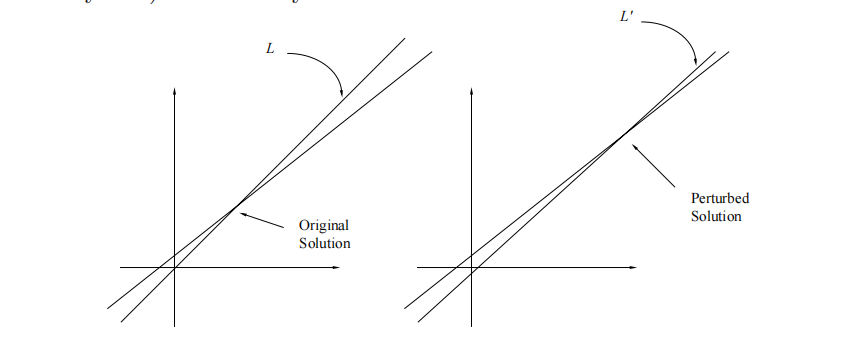
\includegraphics[width=0.8\textwidth]{images/fig1.6.1.png}
    \caption{1.6.1}
    \label{figure1.6.1}
\end{figure}

这在图\ref{figure1.6.1}中得到了说明,其中线 $L$ 被稍微扰动成为线 $L^{\prime}$ 。请注意这个小扰动如何导致交点发生较大变化。这正是例\ref{example1.6.1}中给出的系统的情况。一般来说,病态系统是那些代表几乎平行线、几乎平行平面以及这些概念的概括的系统。

因为舍入误差可以被视为对系统原始系数的扰动,所以即使在病态系统上使用一般良好的数值技术(缺乏精确的算术)也会带来产生无意义结果的风险。

在处理病态系统时,工程师或科学家经常面临比简单地尝试解决系统更基本(有时更令人不安)的问题。即使可以创造一个小奇迹,从而提取出精确的解决方案,科学家或工程师仍然可能得到一个无意义的解决方案,从而导致完全错误的结论。问题源于这样一个事实,即系数通常是凭经验获得的,因此只能在一定的公差范围内得知。对于病态系统,任何系数的微小不确定性都可能意味着解中可能存在极大的不确定性。这种巨大的不确定性甚至可能使精确的解决方案变得毫无用处。

\begin{example}
\label{example1.6.2}
假设方程组:
$$
\begin{cases} 
.835x + .667y = b_1, \\
.333x + .266y = b_2
\end{cases}
$$
中的$b_1$和$b_2$是实验结果,必须从测试仪器的刻度盘上读取。假设刻度盘的读数误差范围为$\pm .001$,且$b_1$和$b_2$的读数分别为$.168$和$.067$,这就构成了示例\ref{example1.6.1}中的病态方程组,并且已知该方程组的精确解为:
\begin{equation}
    (x,y) = (1,-1) \label{equation1.6.1}
\end{equation}
然而,由于刻度盘读数的微小不确定性,我们有:
\begin{equation}
.167 \leq b_1 \leq .169, \quad .066 \leq b_2 \leq .068 \label{equation1.6.2}    
\end{equation}
例如,这意味着读数$(b_1, b_2) = (.168, .067)$对应的解与读数$(b_1, b_2) = (.167, .068)$、$(b_1, b_2) = (.169, .066)$或落在范围(1.6.2)内的任何其他读数对应的解一样有效。对于读数$(b_1, b_2) = (.167, .068)$,精确解为:
\begin{equation}
    (x,y) = (934, -1169) \label{equation1.6.3}
\end{equation}
而对于另一个读数$(b_1, b_2) = (.169, .066)$,精确解为:
\begin{equation}
    (x,y) = (-932, 1167) \label{equation1.6.4}
\end{equation}

你愿意成为第一个乘坐设计中包含该问题解的飞机,或驾驶通过该问题解设计的桥梁的人吗?我不愿意!不确定性太大了。由于解\ref{equation1.6.1}、\ref{equation1.6.3}和\ref{equation1.6.4}中的任何一个都不比其他解更优,因此技术人员如何读取刻度盘上最后一位有效数字,可能会导致采用完全不同的设计方案。由于相关线性方程组的病态性质,飞机或桥梁的成功设计可能取决于运气,而非科学原理。
\end{example}

与其试图从病态方程组中提取精确解,工程师和科学家通常最好将时间和资源投入到重新设计相关实验或数据收集方法上,以避免产生病态方程组。

病态方程组还有另一个令人不安的方面,涉及学生所谓的“检验答案”——将计算出的解代入原方程组的左侧,看它与右侧的接近程度,从而判断解的正确性。更正式地说,若:

$$
x_c = \left(\begin{array}{llll} 
\xi_1 & \xi_2 & \cdots & \xi_n
\end{array}\right)
$$
是方程组:
$$
\begin{cases} 
a_{11}x_1 + a_{12}x_2 + \cdots + a_{1n}x_n = b_1, \\
a_{21}x_1 + a_{22}x_2 + \cdots + a_{2n}x_n = b_2, \\
\vdots \\
a_{n1}x_1 + a_{n2}x_2 + \cdots + a_{nn}x_n = b_n
\end{cases}
$$
的计算解,则称:
$$
r_i = a_{i1}\xi_1 + a_{i2}\xi_2 + \cdots + a_{in}\xi_n - b_i \quad (i = 1, 2, \cdots, n)
$$
为\textbf{残差}。假设你计算出一个解$x_c$,将其代入原方程组后发现所有残差都相对较小,这是否能保证$x_c$接近精确解?令人惊讶的是,当方程组是病态时,答案绝对是否定的!

\begin{example}
\label{example1.6.3}
对于示例\ref{example1.6.3}中的病态方程组,假设你计算出的解为
$$\xi_1 = -666, \quad \xi_2 = 834$$
若你试图通过将其代入原方程组来“检验误差”,使用精确算术计算可得残差:
$$
r_1 = .835\xi_1 + .667\xi_2 - .168 = 0
$$
$$
r_2 = .333\xi_1 + .266\xi_2 - .067 = -.001
$$
也就是说,计算解$(-666, 834)$精确满足第一个方程,且非常接近满足第二个方程。表面上看,这似乎表明计算解应该非常接近精确解。实际上,一个外行甚至可能被误导,认为计算解与精确解的误差在$\pm .001$范围内。显然,事实远非如此,因为精确解是
$$
x = 1, \quad y = -1
$$
对于第一次看到这种情况的学生来说,这总是一个冲击,因为它与新手的直觉相悖。不幸的是,许多学生毕业时仍然认为,通过将计算结果代入原方程,总能“检验”计算的准确性——很高兴你不属于这类学生。
\end{example}

这就引出了一个问题:“如何检验计算解的准确性?”幸运的是,若方程组是良态的,残差确实能更有效地衡量准确性。但这意味着你必须能够回答一些额外的问题,例如:如何预先判断给定的方程组是否是病态的?如何衡量线性方程组的病态程度?

一种确定病态程度的技术可能是:轻微扰动选定的系数,观察解的变化情况。若对某些系数的微小扰动导致解发生显著变化,则说明遇到了病态情况;若某个扰动未导致解发生较大变化,则无法得出结论——可能扰动的是错误的系数集。

通过对不同的系数集进行多次这样的实验,可以对病态程度有一个大致的了解(但不能保证准确)。这种方法成本高昂,且不太令人满意。但在开发出更复杂的工具之前,无法进一步深入讨论。

\begin{exercise}
\label{exercise1.6.1}
考虑示例\ref{example1.6.1}中的病态方程组:
$$
\begin{cases} 
.835x + .667y = .168, \\
.333x + .266y = .067
\end{cases}
$$
\begin{enumerate}[label=(\alph*)]
    \item 描述使用5位算术且不进行尺度变换时,求解该方程组的结果。\label{item1.6.1.a}
    \item 再次使用5位算术,但先对方程组进行行尺度变换,然后再尝试求解,描述这种方法的帮助程度。\label{item1.6.1.b}
    \item 现在使用6位算术且不进行尺度变换,求解该方程组,将结果与精确解进行比较。\label{item1.6.1.c}
    \item 使用6位算术,计算\ref{item1.6.1.c}中解的残差,并解释结果。\label{item1.6.1.d}
    \item 对于(c)中得到的同一个解,此次使用7位算术计算残差,并解释结果。\label{item1.6.1.e}
    \item 总结\ref{item1.6.1.a}到\ref{item1.6.1.e}中的要点,形成结论性陈述。
\end{enumerate}
\end{exercise}

\begin{exercise}
对上述练习\ref{exercise1.6.1}中的病态方程组进行扰动,形成以下方程组:
$$
\begin{cases} 
.835x + .667y = .166995, \\
.333x + .266y = .066995
\end{cases}
$$ 
\begin{enumerate}[label=(\alph*)]
    \item 确定该方程组的精确解,并将其与练习\ref{exercise1.6.1}中方程组的精确解进行比较。\label{item1.6.2.a}
    \item 根据\ref{item1.6.2.a}的结果,就病态方程组的解是否必然会因原方程组的每次扰动而发生显著变化这一问题,形成陈述。
\end{enumerate}
\end{exercise}

\begin{exercise}
考虑由以下两个方程的图像确定的两条直线:
$$
\begin{cases} 
.835x + .667y = .168, \\
.333x + .266y = .067
\end{cases}
$$
\begin{enumerate}[label=(\alph*)]
    \item 使用5位算术计算每条直线的斜率,然后使用6位算术重复计算,在每种情况下,在坐标系中绘制图像。
    \item 通过图形说明,为什么对其中任何一条直线的微小扰动都可能导致解发生较大变化。
    \item 用几何术语描述方程组为最优良态时必须满足的条件。
\end{enumerate}
\end{exercise}

\section{矩阵系统与阶梯形}

% 定义画圈命令,用于标记主元
\newcommand{\circlednum}[1]{%
    \tikz[baseline=(char.base)]{%
        \node[draw, circle, inner sep=1pt] (char) {#1};%
    }%
}

\section{一般线性系统与阶梯形式}
正如我们在前一节中提到的,解线性方程组的方法是将其转化为增广矩阵,使用初等行变换将增广矩阵化简,然后解由简化矩阵表示的等价系统。这个过程如下图所示。

\begin{figure}[h]
    \centering
    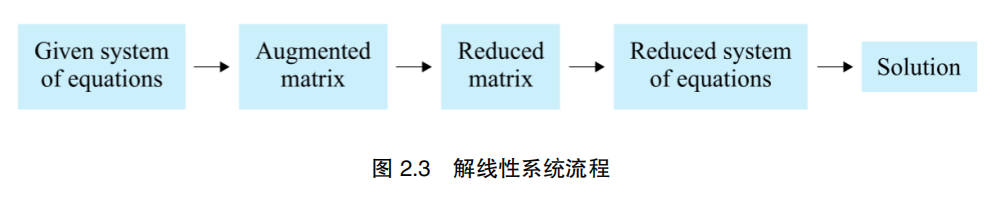
\includegraphics[width=\linewidth]{../images/2.1-1.png} % 请根据实际情况替换图片路径
    \caption{解线性系统流程}
    \label{fig:linear_system_process}
\end{figure}

我们了解了对于 \(n \times n\) 矩阵进行高斯消去的相关内容,这对应于有 \(n\) 个方程和 \(n\) 个未知数的情况。但是如果我们要推广到更一般的线性系统,该如何操作呢?在本节中,我们将介绍更一般的高斯消去法,给出一般线性系统矩阵的行阶梯形式。

我们的第一个目标是将高斯消元技术从方程组扩展到完全通用的矩形系统即线性系统方程的个数与变量的个数不相等的情况。回顾一下,对于具有唯一解的方程组,主元的位置总是位于系数矩阵 \(A\) 的主对角线上- 即从左上角到右下角的对角线上。这样做可以确保高斯消元导致 \(A\) 被减小为一个三角矩阵。以 \(n=4\) 为例,如下图所示:
\[
T=\begin{pmatrix} 
\circledast & * & * & * \\ 
0 & \circledast & * & * \\ 
0 & 0 & \circledast & * \\ 
0 & 0 & 0 & \circledast 
\end{pmatrix}
\]
我们知道主元必须是非零数。对于具有唯一解的方阵系统,我们总是可以在主对角线上的每个关键位置引入一个非零数。然而,在一般矩形系统的情况下,在系数矩阵中并不总是可能使主元位置位于一条直线上。这意味着高斯消去的最终结果不会是三角形的。例如,考虑以下系统:
\[
\begin{cases} 
x_{1}+2 x_{2}+x_{3}+3 x_{4}+3 x_{5}=5 \\ 
2 x_{1}+4 x_{2}+4 x_{4}+4 x_{5}=6 \\ 
x_{1}+2 x_{2}+3 x_{3}+5 x_{4}+5 x_{5}=9 \\ 
2 x_{1}+4 x_{2}+4 x_{4}+7 x_{5}=9 
\end{cases}
\]
该系统的系数矩阵为:
\[
A=\begin{pmatrix} 
1 & 2 & 1 & 3 & 3 \\ 
2 & 4 & 0 & 4 & 4 \\ 
1 & 2 & 3 & 5 & 5 \\ 
2 & 4 & 0 & 4 & 7 
\end{pmatrix}
\]
对系数矩阵 \(A\) 应用高斯消去法得到如下形式:
\[
\begin{pmatrix} 
\circlednum{1} & 2 & 1 & 3 & 3 \\ 
2 & 4 & 0 & 4 & 4 \\ 
1 & 2 & 3 & 5 & 5 \\ 
2 & 4 & 0 & 4 & 7 
\end{pmatrix}
\to
\begin{pmatrix} 
1 & 2 & 1 & 3 & 3 \\ 
0 & \circlednum{0} & -2 & -2 & -2 \\ 
0 & 0 & 2 & 2 & 2 \\ 
0 & 0 & -2 & -2 & 1 
\end{pmatrix}
\]
在之前所讨论的高斯消去的过程中,从第一行开始向下然后向右进行消除,如果向右移动下一个位置进行消除时,此时该位置元素为0,这时则执行与该位置所在行以下的行的交换,以便将非零数带入该位置。但是,在本例中,显然不可能通过将第二行与较低的行互换来将非零数带入 \((2,2)\) 位置。

\subsection{高斯消去法的改进与行阶梯型(Row Echelon Form)}
我们知道在一般矩形系统的情况下,对系数矩阵作高斯消去时在矩阵中并不总是可能使主元位置位于一条对角直线上。这意味着高斯消去的最终结果不会是三角形式。为了处理这种情况,我们对高斯消去做了一定的修改。

\begin{bluebox}{修正后的高斯消元法}
假设 \(U\) 是第 \(i-1\) 步高斯消去后的系统增广矩阵。执行第 \(i\) 步的步骤如下:
\begin{itemize}
    \item 在 \(U\) 中从左到右移动,找到第 \(i\) 个非零位置或该位置下面包含非零元素的那一列,我们把这一列写作 \(U_{* j}\)。
    \item 第 \(i\) 步高斯消去后的主元位置是在 \((i, j)\)。
    \item 如果 \((i, j)\) 的元素为0,则可以将第 \(i\) 行与下面的非零行交换,将一个非零数带入 \((i, j)\) 位置,然后消去这个主元以下的所有元素。
    \item 如果行 \(U_{i *}\) 以及下面 \(U\) 中的所有行都是零,那么消除过程就完成了。
\end{itemize}
\end{bluebox}

% 红色文字
\textcolor{red}{例子2.1.1}
% 红色水平线(宽度为文本宽度,厚度0.4pt)
\color{red}\rule{\textwidth}{0.4pt}\color{black}

对以下矩阵应用修正高斯消去法,圈出支点位置:
\[
A=\begin{pmatrix} 
1 & 2 & 1 & 3 & 3 \\ 
2 & 4 & 0 & 4 & 4 \\ 
1 & 2 & 3 & 5 & 5 \\ 
2 & 4 & 0 & 4 & 7 
\end{pmatrix}
\]
解答:
\[
\begin{pmatrix} 
\circlednum{1} & 2 & 1 & 3 & 3 \\ 
2 & 4 & 0 & 4 & 4 \\ 
1 & 2 & 3 & 5 & 5 \\ 
2 & 4 & 0 & 4 & 7 
\end{pmatrix}
\to
\begin{pmatrix} 
\circlednum{1} & 2 & 1 & 3 & 3 \\ 
0 & 0 & \circlednum{2} & -2 & -2 \\ 
0 & 0 & 2 & 2 & 2 \\ 
0 & 0 & -2 & -2 & 1 
\end{pmatrix}
\]

\[
\to
\begin{pmatrix} 
\circlednum{1} & 2 & 1 & 3 & 3 \\ 
0 & 0 & \circlednum{2} & -2 & -2 \\ 
0 & 0 & 0 & 0 & \circlednum{0} \\ 
0 & 0 & 0 & 0 & 3 
\end{pmatrix}
\to
\begin{pmatrix} 
\circlednum{1} & 2 & 1 & 3 & 3 \\ 
0 & 0 & \circlednum{2} & -2 & -2 \\ 
0 & 0 & 0 & 0 & \circlednum{3} \\ 
0 & 0 & 0 & 0 & 0 
\end{pmatrix}
\]
上面的例子中应用高斯消去的最终结果不是一个纯粹的三角形形式,而是一个锯齿状或"阶梯"类型的三角形形式。此后,具有这种阶梯结构的矩阵将被称为行阶梯形式。

\begin{bluebox}{修正后的高斯消元法}
一个 \(m \times n\) 矩阵 \(E\),其行 \(E_{i *}\),列 \(E_{* j}\) 被称为行阶梯形,满足下面两个条件:
\begin{itemize}
    \item 如果 \(E_{i *}\) 全部由0组成,那么 \(E_{i}\) 下面的所有行也全部为0,即所有的零行都在 \(E\) 底部。
    \item 如果 \(E_{i}\) 中的第一个非零项在第 \(j\) 个位置,那么在这之前的所有列在 \(E_{* 1}, E_{* 2}, \cdots, E_{* j}\) 中第 \(i\) 行位置以下的项全为0。
\end{itemize}
\end{bluebox}

这两个条件说明,行阶梯形中的非零元素必须位于或高于一条阶梯线,这条线从左上角开始,并向右向下倾斜。主元是每一行的第一个非零项。行阶梯形矩阵的典型结构如下图所示:
\[
\begin{pmatrix} 
\circledast & * & * & * & * & * & * & * \\ 
0 & 0 & \circledast & * & * & * & * & * \\ 
0 & 0 & 0 & \circledast & * & * & * & * \\ 
0 & 0 & 0 & 0 & 0 & 0 & \circledast & * \\ 
0 & 0 & 0 & 0 & 0 & 0 & 0 & 0 \\ 
0 & 0 & 0 & 0 & 0 & 0 & 0 & 0 
\end{pmatrix}
\]
由于选择行变换将矩阵 \(A\) 简化为行阶梯形 \(E\) 的灵活性, \(E\) 中的元素不是唯一由 \(A\) 决定的。但是,可以证明 \(E\) 的"形式"是唯一的,因为 \(E(A)\) 中的主元位置是唯一由矩阵 \(A\) 中的元素决定的。因此,主元的个数与 \(E\) 中的非零行数相同,它唯一由 \(A\) 中的元素确定。主元的个数通常成为矩阵 \(A\) 的秩。它在矩阵分析中起到至关重要的作用。

\begin{bluebox}{矩阵的秩(Rank of a Matrix)}
假设矩阵 \(A_{m \times n}\) 通过行变换化为阶梯形 \(E\), 那么矩阵 \(A\) 的秩被定义为下面这个数:
\[
\begin{aligned} 
rank(A) & = \text{矩阵中主元的数量} \\ 
& = \text{矩阵 E 中非零行的数量} \\ 
& = \text{矩阵 A 中的基本列的数量} 
\end{aligned}
\]
其中矩阵 \(A\) 的基本列被定义为 \(A\) 中包含主元位置的列。
\end{bluebox}
 
% 红色文字
\textcolor{red}{例子 2.1.2}
% 红色水平线(宽度为文本宽度,厚度0.4pt)
\color{red}\rule{\textwidth}{0.4pt}\color{black}

Problem: Determine the rank, and identify the basic columns in
\[
A = 
\begin{pmatrix}
1 & 2 & 1 & 1 \\
2 & 4 & 2 & 2 \\
3 & 6 & 3 & 4
\end{pmatrix}
\]

\textbf{Solution:} Reduce \( A \) to row echelon form as shown below:

\[
A = 
\begin{pmatrix}
1 & 2 & 1 & 1 \\
2 & 4 & 2 & 2 \\
3 & 6 & 3 & 4
\end{pmatrix}
\rightarrow
\begin{pmatrix}
1 & 2 & 1 & 1 \\
0 & 0 & 0 & 0 \\
0 & 0 & 0 & 1
\end{pmatrix}
\rightarrow
\begin{pmatrix}
1 & 2 & 1 & 1 \\
0 & 0 & 0 & 1 \\
0 & 0 & 0 & 0
\end{pmatrix}
= E
\]

Consequently, \( \text{rank}(A) = 2 \). The pivotal positions lie in the first and fourth columns so that the basic columns of \( A \) are \( A_{*1} \) and \( A_{*4} \). That is,

\[
\text{Basic Columns} = 
\left\{ 
\begin{pmatrix}
1 \\
2 \\
3
\end{pmatrix},
\begin{pmatrix}
1 \\
2 \\
4
\end{pmatrix}
\right\}
\]

Pay particular attention to the fact that the basic columns are extracted from \( A \) and not from the row echelon form \( E \).

\[
\begin{array}{c}
\text{pivot} \\
\downarrow \\
\begin{pmatrix}
1 & 4 & 5 & -9 & -7 \\
-1 & -2 & -1 & 3 & 1 \\
-2 & -3 & 0 & 3 & -1 \\
0 & -3 & -6 & 4 & 9
\end{pmatrix}\\
\uparrow \text{pivot column}
\end{array}
\]

% 红色文字
\textcolor{red}{练习2.1, 可以参考 ccjou.wordpress.com/2015/03/02/可对角化矩阵的分解篇/ Page 26}
% 红色水平线(宽度为文本宽度,厚度0.4pt)
\color{red}\rule{\textwidth}{0.4pt}\color{black}

\begin{enumerate}[leftmargin=*, label=\bfseries 2.1.\arabic*]

\item Reduce each of the following matrices to row echelon form, determine the rank, and identify the basic columns.

\begin{enumerate}[label=(\alph*)]
    \item $\begin{pmatrix}
        1 & 2 & 3 & 3 \\
        2 & 4 & 6 & 9 \\
        2 & 6 & 7 & 6
    \end{pmatrix}$
    
    \item $\begin{pmatrix}
        1 & 2 & 3 \\
        2 & 6 & 8 \\
        2 & 6 & 0 \\
        1 & 2 & 5 \\
        3 & 8 & 6
    \end{pmatrix}$
    
    \item $\begin{pmatrix}
        2 & 1 & 1 & 3 & 0 & 4 & 1 \\
        4 & 2 & 4 & 4 & 1 & 5 & 5 \\
        2 & 1 & 3 & 1 & 0 & 4 & 3 \\
        6 & 3 & 4 & 8 & 1 & 9 & 5 \\
        0 & 0 & 3 & -3 & 0 & 0 & 3 \\
        8 & 4 & 2 & 14 & 1 & 13 & 3
    \end{pmatrix}$
\end{enumerate}

\item Determine which of the following matrices are in row echelon form:

\begin{enumerate}[label=(\alph*)]
    \item $\begin{pmatrix}
        1 & 2 & 3 \\
        0 & 0 & 4 \\
        0 & 1 & 0
    \end{pmatrix}$
    
    \item $\begin{pmatrix}
        0 & 0 & 0 & 0 \\
        0 & 1 & 0 & 0 \\
        0 & 0 & 0 & 1
    \end{pmatrix}$
    
    \item $\begin{pmatrix}
        2 & 2 & 3 & -4 \\
        0 & 0 & 7 & -8 \\
        0 & 0 & 0 & -1
    \end{pmatrix}$
    
    \item $\begin{pmatrix}
        1 & 2 & 0 & 0 & 1 & 0 \\
        0 & 0 & 0 & 1 & 0 & 0 \\
        0 & 0 & 0 & 0 & 0 & 1 \\
        0 & 0 & 0 & 0 & 0 & 0
    \end{pmatrix}$
\end{enumerate}

\item Suppose that \( A \) is an \( m \times n \) matrix. Give a short explanation of why each of the following statements is true.

\begin{enumerate}[label=(\alph*)]
    \item \(\text{rank}(A) \leq \min\{m, n\}\).
    
    \item \(\text{rank}(A) < m\) if one row in \( A \) is entirely zero.
    
    \item \(\text{rank}(A) < m\) if one row in \( A \) is a multiple of another row.
    
    \item \(\text{rank}(A) < m\) if one row in \( A \) is a combination of other rows.
    
    \item \(\text{rank}(A) < n\) if one column in \( A \) is entirely zero.
\end{enumerate}

\item Let \( A = \begin{pmatrix}
    .1 & .2 & .3 \\
    .4 & .5 & .6 \\
    .7 & .8 & .901
\end{pmatrix} \).

\begin{enumerate}[label=(\alph*)]
    \item Use exact arithmetic to determine \(\text{rank}(A)\).
    
    \item Now use 3-digit floating-point arithmetic (without partial pivoting or scaling) to determine \(\text{rank}(A)\). This number might be called the "3-digit numerical rank."
    
    \item What happens if partial pivoting is incorporated?
\end{enumerate}

\item How many different "forms" are possible for a \( 3 \times 4 \) matrix that is in row echelon form?

\item Suppose that \([A | b]\) is reduced to a matrix \([E | c]\).

\begin{enumerate}[label=(\alph*)]
    \item Is \([E | c]\) in row echelon form if \( E \) is?
    
    \item If \([E | c]\) is in row echelon form, must \( E \) be in row echelon form?
\end{enumerate}

\end{enumerate}



\subsection*{2.2 行简化阶梯形矩阵(REDUCED ROW ECHELON FORM)}

在 2.1 节中,我们引入了行阶梯形的概念。若在高斯-约当消元法的基础上再施加两个额外的条件,我们将得到一种形式更简洁、性质更优良的矩阵,称为\textbf{行简化阶梯形矩阵}。

\subsubsection*{2.2.1行简化阶梯形的定义}

一个 \( m \times n \) 的矩阵 \( E \) 被称为是\textbf{行简化阶梯形},当且仅当它满足以下三个条件:
\begin{enumerate}
    \item \( E \) 是行阶梯形矩阵。
    \item \textbf{每个主元(即每行第一个非零元素)均为 1}。
    \item \textbf{每个主元所在的列中,除主元自身外,其他所有元素均为 0}。
\end{enumerate}

行简化阶梯形矩阵的典型结构如下所示,其中标有 \(*\) 的元素可以是任意数(零或非零):

\[
E = \begin{pmatrix}
1 & * & 0 & 0 & * & * & 0 & * \\
0 & 0 & 1 & 0 & * & * & 0 & * \\
0 & 0 & 0 & 1 & * & * & 0 & * \\
0 & 0 & 0 & 0 & 0 & 0 & 1 & * \\
0 & 0 & 0 & 0 & 0 & 0 & 0 & 0 \\
0 & 0 & 0 & 0 & 0 & 0 & 0 & 0
\end{pmatrix}
\]

\subsubsection*{2.2.2行简化阶梯形的唯一性}

行简化阶梯形一个至关重要的性质是其\textbf{唯一性}。
\begin{itemize}
    \item 对于任意矩阵 \( A \),无论采用何种初等行变换序列将其化简,最终得到的行简化阶梯形矩阵 \( E_A \) 都是\textbf{唯一确定}的。
    \item 这种唯一性使得 \( E_A \) 在理论分析中非常有用,它可以作为一个"地图"或"密钥",来揭示原始矩阵 \( A \) 的列向量之间隐藏的线性关系。
\end{itemize}

\subsubsection*{2.2.3列关系在 \( E_A \) 与 \( A \) 中的体现}

在简化形式 \( E_A \) 中,列向量之间的关系是清晰透明的:
\begin{itemize}
    \item 每一个非基本列 \( E_{*k} \) 都可以表示为位于其左侧的基本列 \( E_{*b_1}, E_{*b_2}, \dots, E_{*b_j} \) 的线性组合:
    \[
    E_{*k} = \mu_1 E_{*b_1} + \mu_2 E_{*b_2} + \cdots + \mu_j E_{*b_j}
    \]
    其中,系数 \( \mu_1, \mu_2, \dots, \mu_j \) 恰好就是向量 \( E_{*k} \) 中的前 \( j \) 个分量。
    
    \item \textbf{关键洞察}:存在于 \( E_A \) 的列之间的这种线性依赖关系,与原始矩阵 \( A \) 的列之间的依赖关系\textbf{完全一致}。因此,若在 \( E_A \) 中有:
    \[
    E_{*k} = \mu_1 E_{*b_1} + \mu_2 E_{*b_2} + \cdots + \mu_j E_{*b_j}
    \]
    那么在 \( A \) 中,必然有:
    \[
    A_{*k} = \mu_1 A_{*b_1} + \mu_2 A_{*b_2} + \cdots + \mu_j A_{*b_j}
    \]
\end{itemize}

% 红色文字
\textcolor{red}{例子2.2.1}
% 红色水平线(宽度为文本宽度,厚度0.4pt)
\color{red}\rule{\textwidth}{0.4pt}\color{black}\\
将矩阵 \( A \) 的每个非基本列表示为基本列的线性组合。
\[
A = \begin{pmatrix}
2 & -4 & -8 & 6 & 3 \\
0 & 1 & 3 & 2 & 3 \\
3 & -2 & 0 & 0 & 8
\end{pmatrix}
\]

解答:
通过初等行变换将 \( A \) 化为行简化阶梯形 \( E_A \):
\[
\begin{pmatrix}
2 & -4 & -8 & 6 & 3 \\
0 & 1 & 3 & 2 & 3 \\
3 & -2 & 0 & 0 & 8
\end{pmatrix}
\rightarrow \cdots \rightarrow
\begin{pmatrix}
1 & 0 & 2 & 0 & 4 \\
0 & 1 & 3 & 0 & 2 \\
0 & 0 & 0 & 1 & \frac{1}{2}
\end{pmatrix} = E_A
\]

在 \( E_A \) 中,第 1, 2, 4 列是基本列。观察非基本列:
\begin{itemize}
    \item \( E_{*3} = 2E_{*1} + 3E_{*2} \)
    \item \( E_{*5} = 4E_{*1} + 2E_{*2} + \frac{1}{2}E_{*4} \)
\end{itemize}

因此,在原始矩阵 \( A \) 中,同样的关系成立:
\begin{itemize}
    \item \( A_{*3} = 2A_{*1} + 3A_{*2} \)
    \item \( A_{*5} = 4A_{*1} + 2A_{*2} + \frac{1}{2}A_{*4} \)
\end{itemize}

可以通过直接计算验证这些等式的正确性。

总结:行简化阶梯形 \( E_A \) 的效用在于它能清晰地揭示出以矩阵列形式存储的数据之间的内在依赖关系,这是普通行阶梯形所不具备的强大理论工具。

% 红色文字
\textcolor{red}{练习2.2}
% 红色水平线(宽度为文本宽度,厚度0.4pt)
\color{red}\rule{\textwidth}{0.4pt}\color{black}

\begin{enumerate}[leftmargin=*, label=\bfseries 2.2.\arabic*]

\item Determine the reduced row echelon form for each of the following matrices and then express each nonbasic column in terms of the basic columns:
\begin{enumerate}[label=(\alph*)]
    \item \(\begin{pmatrix}
        1 & 2 & 3 & 3 \\
        2 & 4 & 6 & 9 \\
        2 & 6 & 7 & 6 
    \end{pmatrix}\)
    
    \item \(\begin{pmatrix}
        2 & 1 & 1 & 3 & 0 & 4 & 1 \\
        4 & 2 & 4 & 4 & 1 & 5 & 5 \\
        2 & 1 & 3 & 1 & 0 & 4 & 3 \\
        6 & 3 & 4 & 8 & 1 & 9 & 5 \\
        0 & 0 & 3 & -3 & 0 & 0 & 3 \\
        8 & 4 & 2 & 14 & 1 & 13 & 3 
    \end{pmatrix}\)
\end{enumerate}

\item Construct a matrix \( A \) whose reduced row echelon form is
\[
E_A = \begin{pmatrix}
1 & 2 & 0 & -3 & 0 & 0 & 0 \\
0 & 0 & 1 & -4 & 0 & 1 & 0 \\
0 & 0 & 0 & 0 & 1 & 0 & 0 \\
0 & 0 & 0 & 0 & 0 & 0 & 1 \\
0 & 0 & 0 & 0 & 0 & 0 & 0 \\
0 & 0 & 0 & 0 & 0 & 0 & 0 
\end{pmatrix}.
\]
Is \( A \) unique?

\item Suppose that \( A \) is an \( m \times n \) matrix. Give a short explanation of why \( \text{rank}(A) < n \) whenever one column in \( A \) is a combination of other columns in \( A \).

\item Consider the following matrix:
\[
A = \begin{pmatrix}
.1 & .2 & .3 \\
.4 & .5 & .6 \\
.7 & .8 & .901 
\end{pmatrix}.
\]
\begin{enumerate}[label=(\alph*)]
    \item Use exact arithmetic to determine \( E_A \).
    \item Now use 3-digit floating-point arithmetic (without partial pivoting or scaling) to determine \( E_A \) and formulate a statement concerning "near relationships" between the columns of \( A \).
\end{enumerate}

\item Consider the matrix
\[
E = \begin{pmatrix}
1 & 0 & -1 \\
0 & 1 & 2 \\
0 & 0 & 0 
\end{pmatrix}.
\]
You already know that \( E_{*3} \) can be expressed in terms of \( E_{*1} \) and \( E_{*2} \). However, this is not the only way to represent the column dependencies in \( E \). Show how to write \( E_{*1} \) in terms of \( E_{*2} \) and \( E_{*3} \) and then express \( E_{*2} \) as a combination of \( E_{*1} \) and \( E_{*3} \).

\noindent \textbf{Note:} This exercise illustrates that the set of pivotal columns is not the only set that can play the role of "basic columns." Taking the basic columns to be the ones containing the pivots is a matter of convenience because everything becomes automatic that way.

\end{enumerate}


\subsection{2.3 线性方程组的一致性(Consistency Of Linear Systems)}

如果一个包含 \(n\) 个未知数的 \(m\) 个线性方程组至少有一个解,则称其为相容方程组。如果没有解,则该方程组
被称为不相容方程组。本节旨在确定给定方程组相容的条件。

对于仅包含两个或三个未知数的方程组,
说明其相容性条件很容易。两个未知数的线性方程表示二维空间中的一条直线,
而三个未知数的线性方程表示三维空间中的平面。因此,
一个包含 \(m\) 个两个未知数的线性方程组相容当且仅当这 \(m\) 个方程定义的 \(m\) 条直线至少有一个公共交点。
同样,一个包含 \(m\) 个三个未知数的方程组相容当且仅当
相关的 \(m\) 个平面至少有一个公共交点。
然而,当 \(m\) 较大时,这些几何条件可能不易直观验证,而当 \(n\) > 3 时,相交线或平面的推广则无法用肉眼直观地看到。

我们不依赖几何来建立一致性,而是使用高斯消元法。如果将相关的增广矩阵 \([\mathbf{A}|\mathbf{b}]\) 通过行运算简化为行阶梯矩阵 \([\mathbf{E}|\mathbf{c}]\),则一致性(或不一致性)变得显而易见。
假设在将 \([\mathbf{A}|\mathbf{b}]\) 简化为 \([\mathbf{E}|\mathbf{c}]\) 的过程中,出现这样一种情况:一行中唯一的非零项出现在右侧,如下所示:

\[
\text{Row }i \rightarrow 
\left(\begin{array}{cccccc|c}
* & * & * & * & * & * & * \\ 
0 & 0 & 0 & * & * & * & * \\ 
0 & 0 & 0 & 0 & 0 & 0 & \alpha \\
\bullet & \bullet & \bullet & \bullet & \bullet & \bullet & \bullet \\
\bullet & \bullet & \bullet & \bullet & \bullet & \bullet & \bullet \\
\end{array}\right)
\leftarrow \alpha \neq 0.
\]

如果这发生在第 \(i\) 行,则相关系统的第 \(i\) 个方程为

\[
0x_1 + 0x_2 + ... + 0x_n = \alpha.
\]

当 \(\alpha \neq 0\) 时,该方程无解,因此原系统也必然不一致(因为行运算不会改变解集)。
反之亦然。也就是说,如果一个系统不一致,那么在消元过程中,会出现如下形式的行

\[
\left(\begin{array}{cccccc|c}
0 & 0 & ... & 0 & \alpha
\end{array}\right), \alpha \neq 0.
\]

否则,回代过程可以完成,并产生一个解。当遇到形式为
(0 0 ... 0 \(\mid\) 0) 的行时,不会指示不一致性。这只是表示 0 = 0,
尽管这对于确定任何未知数的值没有任何帮助,但它仍然是一个真实的陈述,
因此它并不表示系统存在不一致。

还有一些其他方法可以表征系统的一致性(或不一致性)。其中一种方法是:如果增广矩阵 \([\mathbf{A}|\mathbf{b}]\) 的最后一列 \(b\) 是非基列,则最后一列不可能存在主元,因此系统是一致的,因为 (2.3.1) 的情况不会发生。
反之,如果系统是一致的,那么 (2.3.1) 的情况在高斯消元法中永远不会发生,因此最后一列不可能是基列。换句话说,\([\mathbf{A}|\mathbf{b}]\) 是一致的当且仅当 \(b\) 是非基列。

说 b 是 \([\mathbf{A}|\mathbf{b}]\) 中的非基列,等同于说\([\mathbf{A}|\mathbf{b}]\) 中的所有基列都位于系数矩阵 A 中。由于矩阵中基列的数量就是秩,因此一致性也可以这样来描述:
当且仅当 rank\([\mathbf{A}|\mathbf{b}]\) = rank\((\mathbf{A})\) 时,系统才是一致的。

\begin{bluebox}{线性方程组的一致性}
满足以下任意一个条件都可以说 \([\mathbf{A}|\mathbf{b}]\) 是一致的:
\begin{itemize}
    \item 行简化阶梯形矩阵 \([\mathbf{A}|\mathbf{b}]\) 中不存在形如下列的行:
    \[
    \left(\begin{array}{cccc|c}
        0 & 0 & ... & 0 & \alpha
    \end{array}\right), \alpha \neq 0
    \]
    \item \(\mathbf{b}\) 是 \([\mathbf{A}|\mathbf{b}]\) 中的非基列。
    \item rank\([\mathbf{A}|\mathbf{b}]\) = rank\((\mathbf{A})\)
    \item \(\mathbf{b}\) 是 \(\mathbf{A}\) 的基列的一个组合。
\end{itemize}
\end{bluebox}

% 红色文字
\textcolor{red}{例子2.3.1}
% 红色水平线(宽度为文本宽度,厚度0.4pt)
\color{red}\rule{\textwidth}{0.4pt}\color{black}

\textbf{问题}: 确定以下系统是否一致: 
\[
\begin{aligned} 
    x_1 + x_2 + 2x_3 + 2x_4 + x_5 &= 1, \\
    2x_1 + 2x_2 + 4x_3 + 4x_4 + 3x_5 &= 1, \\
    2x_1 + 2x_2 + 4x_3 + 4x_4 + 2x_5 &= 2, \\
    3x_1 + 5x_2 + 8x_3 + 6x_4 + 5x_5 &= 3.
\end{aligned}
\]
\textbf{解答}: 对增广矩阵 \([\mathbf{A}|\mathbf{b}]\) 应用高斯消元法,如下所示
\[
\left(\begin{array}{ccccc|c} 
\circlednum{1} & 1 & 2 & 2 & 1 & 1 \\ 
2 & 2 & 4 & 4 & 3 & 1 \\ 
2 & 2 & 4 & 4 & 2 & 2 \\ 
3 & 5 & 8 & 6 & 5 & 3 
\end{array}\right)
\to
\left(\begin{array} {ccccc|c} 
\circlednum{1} & 1 & 2 & 2 & 1 & 1 \\ 
0 & \circlednum{0} & 0 & 0 & 1 & -1 \\ 
0 & 0 & 0 & 0 & 0 & 0 \\ 
0 & 2 & 2 & 0 & 2 & 0 
\end{array}\right)
\to
\left(\begin{array}{ccccc|c} 
\circlednum{1} & 1 & 2 & 2 & 1 & 1 \\ 
0 & \circlednum{2} & 2 & 0 & 2 & 0 \\ 
0 & 0 & 0 & 0 & \circlednum{1} & -1 \\ 
0 & 0 & 0 & 0 & 0 & 0 
\end{array}\right)
\]

由于形式为 \(\left(\begin{array}{cccc|c} 0 & 0 & \dots & 0 & \alpha \end{array}\right),\ \alpha \neq 0\) 的行从未出现,
因此系统是一致的。我们还可以观察到,\(b\) 是 \([\mathbf{A}|\mathbf{b}]\) 中的非基本列,
因此 rank\([\mathbf{A}|\mathbf{b}]\) = rank \((\mathbf{A})\)。最后,通过将 \(\mathbf{A}\) 完全约化为
\(\mathbf{E_A}\),可以验证 \(\mathbf{b}\) 确实是基本列的组合,\{\(\mathbf{A_{*1}}, \mathbf{A_{*2}}, \mathbf{A_{*5}}\)\}。

% 红色文字
\textcolor{red}{练习 2.3}
% 红色水平线(宽度为文本宽度,厚度0.4pt)
\color{red}\rule{\textwidth}{0.4pt}\color{black}

\begin{enumerate}[leftmargin=*, label=\bfseries 2.3.\arabic*]

\item Determine which of the following systems are consistent.

\begin{enumerate}[label=(\alph*)]
    \item \(\begin{array}{l}
    x + 2y + z = 2, \\
    2x + 4y = 4, \\
    3x + 6y + z = 4.
    \end{array}\)
    
    \item \(\begin{array}{l}
    2x + 2y + 4z = 0, \\
    3x + 2y + 5z = 0, \\
    4x + 2y + 6z = 0.
    \end{array}\)
    
    \item \(\begin{array}{l}
    x - y + z = 1, \\
    x - y - z = 2, \\
    x + y - z = 3, \\
    x + y + z = 4.
    \end{array}\)

    \item \(\begin{array}{l}
    x - y + z = 1, \\
    x - y - z = 2, \\
    x + y - z = 3, \\
    x + y + z = 2.
    \end{array}\)

    \item \(\begin{array}{l}
    2w + x + 3y + 5z = 1, \\
    4w + 4y + 8z = 0, \\
    w + x + 2y + 3z = 0, \\
    x + y + z = 0.
    \end{array}\)

    \item \(\begin{array}{l}
    2w + x + 3y + 5z = 7, \\
    4w + 4y + 8z = 8, \\
    w + x + 2y + 3z = 5, \\
    x + y + z = 3.
    \end{array}\)
\end{enumerate}

\item Construct a \(3 \times 4\) matrix \(A\) and \(3 \times 1\) columns \(b\) and \(c\) such that \([\mathbf{A}|\mathbf{b}]\) is the augmented matrix for an inconsistent system, but \([\mathbf{A}|\mathbf{c}]\) is the augmented matrix for a consistent system.

\item If \(\mathbf{A}\) is an \(m \times n\) matrix with rank\((\mathbf{A}) = m\), explain why the system \([\mathbf{A}|\mathbf{b}]\) must be consistent for every right-hand side \(\mathbf{b}\).

\item Is it possible for a parabola whose equation has the form \(y = \alpha+\beta x+\gamma x^2\) to pass through the four points (0, 1), (1, 3), (2, 15), and (3, 37)? Why?

\item Consider using floating-point arithmetic (without scaling) to solve the following system:
\[
\begin{array}{l}
.835x + .667y = .168, \\
.333x + .266y = .067.
\end{array}
\]
\begin{enumerate}[label=(\alph*)]
    \item Is the system consistent when 5-digit arithmetic is used?
    
    \item What happens when 6-digit arithmetic is used?
\end{enumerate}

\item In order to grow a certain crop, it is recommended that each square foot of ground be treated with 10 units of phosphorous, 9 units of potassium, and 19 units of nitrogen. 
Suppose that there are three brands of fertilizer on the market— say brand \(\mathcal{X}\) , brand \(\mathcal{Y}\) , and brand \(\mathcal{Z}\).
One pound of brand \(\mathcal{X}\) contains 2 units of phosphorous, 3 units of potassium, and 5 units of nitrogen. One pound of brand \(\mathcal{Y}\) contains 1 unit of phosphorous,
3 units of potassium, and 4 units of nitrogen. One pound of brand \(\mathcal{Z}\) contains only 1 unit of phosphorous and 1 unit of nitrogen.
Determine whether or not it is possible to meet exactly the recommendation by applying some combination of the three brands of fertilizer.

\item Suppose that an augmented matrix \([\mathbf{A}|\mathbf{b}]\) is reduced by means of Gaussian elimination to a row echelon form \([\mathbf{E}|\mathbf{c}]\). If a row of the form 
\[
\left(\begin{array}{cccc|c}
    0 & 0 & ... & 0 & \alpha
\end{array}\right), \alpha \neq 0
\]
does not appear in \([\mathbf{E}|\mathbf{c}]\), is it possible that rows of this form could have appeared at earlier stages in the reduction process? Why?

\end{enumerate}

\subsection{2.4 齐次系统(Homogeneous Systems)}

\(n\) 个未知数的 \(m\) 个线性方程组
\[
\begin{array}{c}
    a_{11}x_1 + a_{12}x_2 + ... + a_{1n}x_n = 0, \\
    a_{21}x_1 + a_{22}x_2 + ... + a_{2n}x_n = 0, \\
    \vdots \\
    a_{m1}x_1 + a_{m2}x_2 + ... + a_{mn}x_n = 0.
\end{array}
\]

如果方程式的右侧完全由0组成,则称其为\textbf{齐次系统}。如果方程式的右侧至少有一个非零数,则该系统称为\textbf{非齐次系统}。本节旨在探讨齐次系统的一些基本概念。

在处理齐次方程组时,一致性从来都不是问题,因为无论系数值如何,
零解 \(x_1 = x_2 = ... = x_n = 0\) 始终是唯一解。下文中,
将全零组成的解称为\textbf{平凡解}。唯一的问题是:“除了平凡解之外,还有其他解吗?
如果有,我们如何才能最好地描述它们?” 和之前一样,高斯消元法可以给出答案。

使用高斯消元法将齐次系统的增广矩阵 \([\mathbf{A|0}]\) 化简为行阶梯形时,右侧的零列不会被任何三种基本行运算改变。
也就是说,任何通过行运算从 \([\mathbf{A|0}]\) 导出的行阶梯形,也必然具有 \([\mathbf{E|0}]\) 的形式。这意味着最后一列的零只是
多余的负担,没有必要在每一步都带上去。只需将系数矩阵 \(\mathbf{A}\) 化简为行阶梯形 \(\mathbf{E}\),并记住在执行回代时,右侧
完全为零。通过一个典型的例子,可以更好地理解这个过程。

为了求解齐次系统的解
\[
\begin{array}{c}
    x_1 + 2x_2 + 2x_3 + 3x_4 = 0, \\
    2x_1 + 4x_2 + x_3 + 3x_4 = 0, \\
    3x_1 + 6x_2 + x_3 + 4x_4 = 0,
\end{array}
\]
将系数矩阵简化为行阶梯形式。
\[
\mathbf{A} = 
\left(\begin{array}{cccc}
1 & 2 & 2 & 3 \\
2 & 4 & 1 & 3 \\
3 & 6 & 1 & 4
\end{array}\right)\to
\left(\begin{array}{cccc}
1 & 2 & 2 & 3 \\
0 & 0 & -3 & -3 \\
0 & 0 & -5 & -5
\end{array}\right)\to
\left(\begin{array}{cccc}
1 & 2 & 2 & 3 \\
0 & 0 & -3 & -3 \\
0 & 0 & 0 & 0
\end{array}\right)
= \mathbf{E}.
\]
因此,原始齐次系统等价于以下简化齐次系统:
\[
\begin{aligned}
    x_1 + 2x_2 + 2x_3 + 3x_4 &= 0, \\
    -3x_3 - 3x_4 &= 0.
\end{aligned}
\]
由于这个简化系统中有四个未知数,但只有两个方程,因此不可能为每个未知数求出唯一的解。我们能做的最好的事情是,
选择两个“基本”未知数——我们称之为\textbf{基本变量},并用另外两个未知数来求解它们——这两个未知数的值必须
保持任意或“自由”,因此它们被称为\textbf{自由变量}。虽然选择一组基本变量有多种可能性,但惯例是始终求解与枢轴位置对应的未知数,
或者,等价地,与基本列对应的未知数。在这个例子中,枢轴(以及基本列)位于第一和第三位置,
因此策略是应用回代法,用自由变量 \(x_2\) 和 \(x_4\) 来求解简化系统中的基本变量 \(x_1\) 和 \(x_3\)。由第二个方程得出
\[
x_3 = -x_4.
\]
代入第一个方程可得
\[
\begin{aligned}
x_1 &= -2x_2 -2x_3 - 3x_4, \\
&= -2x_2 - 2(-x_4) - 3x_4, \\
&= -2x_2 - x_4.
\end{aligned}
\]
因此,原齐次系统的所有解都可以描述为
\[
\begin{aligned}
    &x_1 = -2x_2 - x_4 \\
    &x_2 \text{ 任意}, \\
    &x_3 = -x_4, \\
    &x_4 \text{ 任意}.
\end{aligned}
\]
由于自由变量 \(x_2\) 和 \(x_4\) 取值范围涵盖所有可能值,上述表达式描述了所有可能的解。例如,当 \(x_2\) 和 \(x_4\) 取值
\(x_2 = 1\) 且 \(x_4 = -2\) 时,则有特定解
\[
x_1 = 0, x_2 = 1, x_3 = 2, x_4 = -2
\]
将来不再像上述那样描述解集,而是更方便地通过以下方式表达解集: 
\[
\left(\begin{array}{c}
x_1\\
x_2\\
x_3\\
x_4
\end{array}\right)=
\left(\begin{array}{c}
-2x_2 - x_4\\
x_2\\
-x_4\\
x_4
\end{array}\right)=
x_2\left(\begin{array}{c}
-2\\
1\\
0\\
0
\end{array}\right)+
x_4\left(\begin{array}{c}
-1\\
0\\
-1\\
1
\end{array}\right)
\]
假设 \(x_2\) 和 \(x_4\) 是自由变量,其取值范围为所有可能的数字。这种表示被称为齐次系统的\textbf{通解}。
通解的表达式强调,每个解都是两个特解的某种组合
\[
\mathbf{h}_1 = 
\left(\begin{array}{c}
-2\\
1\\
0\\
0
\end{array}\right),  
\mathbf{h}_2 =
\left(\begin{array}{c}
-1\\
0\\
-1\\
1
\end{array}\right).
\]
\(\mathbf{h}_1\) 和 \(\mathbf{h}_2\) 显然都是解,因为 \(\mathbf{h}_1\) 是在自由变量取值 \(x_2 = 1\) 和 \(x_4 = 0\) 时生成的,而
解 \(\mathbf{h}_2\) 是在 \(x_2 = 0\) 和 \(x_4 = 1\) 时生成的。

现在考虑一个由 \(m\) 个线性方程组 \([\mathbf{A|0}]\) 组成的广义齐次方程组,
其中有 \(n\) 个未知数。如果系数矩阵的 rank(\(\mathbf{A}\)) = \(r\),那么
从前面的讨论中应该可以明显看出,恰好有 \(r\) 个
基本变量(对应于 \(\mathbf{A}\) 中基本列的位置),以及
恰好有 \(n - r\) 个自由变量(对应于 \(\mathbf{A}\) 中非基本列的位置)。
使用高斯消元法将 \(\mathbf{A}\) 化为行阶梯形,
然后使用回代法根据自由变量求解基本变量,
即可得到\textbf{通解},其形式为
\[
\mathrm{x} = x_{f_1}\mathbf{h}_1 + x_{f_2}\mathbf{h}_2 + ... + x_{f_{n-r}}\mathbf{h}_{n-r},
\]
其中 \(x_{f_1}, x_{f_2}, ..., x_{f_{n-r}}\) 为自由变量,\(\mathbf{h}_1, \mathbf{h}_2, ..., \mathbf{h}_{n-r}\) 为
\(n \times 1\) 列,表示系统的特定解。由于自由变量 \(x_{f_i}\) 涵盖所有可能值,因此通解会生成所有可能的解。

通解并不依赖于所用的行阶梯形式,因为无论使用哪种行阶梯形式,使用回代法求解基本变量,都会生成一组唯一的特解,
{\(\mathbf{h}_1, \mathbf{h}_2, ..., \mathbf{h}_{n-r}\)}。无需赘述,我们可以认为这是正确的,因为使用任何行阶梯形式求解基本变量,
其结果必然与将 \(\mathbf{A}\) 完全简化为 \(\mathbf{E_A}\),然后求解简化齐次系统的基本变量,所得结果完全相同。\(\mathbf{E_A}\) 的唯一性,保证了 \(\mathbf{h}_i\) 的唯一性。

例如,如果与第一个系统相关的系数矩阵 \(\mathbf{A}\) 通过高斯-乔丹方法完全简化为 \(\mathbf{E_A}\)
\[
\mathbf{A} = 
\left(\begin{array}{cccc}
    1 & 2 & 2 & 3 \\
    2 & 4 & 1 & 3 \\
    3 & 6 & 1 & 4 \\
\end{array}\right)\to
\left(\begin{array}{cccc}
    1 & 2 & 0 & 1 \\
    0 & 0 & 1 & 1 \\
    0 & 0 & 0 & 0 \\
\end{array}\right)= \mathbf{E_A}
\]
然后我们得到以下简化系统:
\[
\begin{aligned}
    x_1 + 2x_2 + x_4 &= 0, \\
    x_3 + x_4 &= 0.
\end{aligned}
\]
用 \(x_2\) 和 \(x_4\) 来求解基本变量 \(x_1\) 和 \(x_3\),得到的结果与当时的推导给出的结果完全相同,因此也得到了与后续的通解完全相同的结果。

由于避免了回代过程,你可能会发现使用高斯-约当法将 \(\mathbf{A}\) 完全简化为 \(\mathbf{E_A}\) 更为方便,
然后直接从 \(\mathbf{E_A}\) 中的元素构建通解。这种方法通常会在示例和练习中采用。

如前所述,所有齐次系统都是一致的,因为由全零组成的平凡解始终是唯一解。一个自然而然的问题是:“平凡解何时是唯一解?”
换句话说,我们想知道齐次系统何时具有唯一解。上述的形式使答案显而易见。只要至少有一个自由变量,那么从上述可以清楚地看出,
将存在无数个解。因此,当且仅当没有自由变量时,平凡解才是唯一解。
由于自由变量的数量为 \(n - r\),其中 \(r\) = rank(\(\mathbf{A}\)),因此前面的陈述可以重新表述为:当且仅当 rank(\(\mathbf{A}\)) = \(n\),齐次系统才具有唯一解——平凡解。

% 红色文字
\textcolor{red}{例子2.4.1}
% 红色水平线(宽度为文本宽度,厚度0.4pt)
\color{red}\rule{\textwidth}{0.4pt}\color{black}

齐次系统
\[
\begin{aligned} 
    x_1 + 2x_2 + 2x_3 = 0, \\
    2x_1 + 5x_2 + 7x_3 = 0, \\
    3x_1 + 6x_2 + 8x_3 = 0.
\end{aligned}
\]
只有平凡解因为
\[
\mathbf{A} = 
\left(\begin{array}{ccc}
    1 & 2 & 2 \\
    2 & 5 & 7 \\
    3 & 6 & 8 \\
\end{array}\right)\to
\left(\begin{array}{cccc}
    1 & 2 & 2 \\
    0 & 1 & 3 \\
    0 & 0 & 2 \\
\end{array}\right) = \mathbf{E}
\]
表明 rank(\(\mathbf{A}\)) = \(n\) = 3。事实上,从 \(\mathbf{E}\) 中也可以看出,在系统 \([\mathbf{E|0}]\) 中应用反向替换只会产生平凡解。

% 红色文字
\textcolor{red}{例子2.4.2}
% 红色水平线(宽度为文本宽度,厚度0.4pt)
\color{red}\rule{\textwidth}{0.4pt}\color{black}

\textbf{问题}: 解释为什么下列齐次系统有无穷多个解,并给出通解:
\[
\begin{aligned} 
    x_1 + 2x_2 + 2x_3 = 0, \\
    2x_1 + 5x_2 + 7x_3 = 0, \\
    3x_1 + 6x_2 + 6x_3 = 0.
\end{aligned}
\]
\textbf{解答}: 
\[
\mathbf{A} = 
\left(\begin{array}{ccc}
    1 & 2 & 2 \\
    2 & 5 & 7 \\
    3 & 6 & 6 \\
\end{array}\right)\to
\left(\begin{array}{cccc}
    1 & 2 & 2 \\
    0 & 1 & 3 \\
    0 & 0 & 0 \\
\end{array}\right) = \mathbf{E}
\]
表明 rank(\(\mathbf{A}\)) = 2 < \(n\) = 3。由于基本列位于位置1 和 2,\(x_1\) 和 \(x_2\) 是基本变量,而 \(x_3\) 是自由变量。使用
\([E|0]\) 的反向代入,用自由变量来求解基本变量,可得 \(x_2 = -3x_3\) 和 \(x_1 = -2x_2 - 2x_3 = 4x_3\),因此通解为
\[
\left(\begin{array}{c}
    x_1 \\
    x_2 \\
    x_3 \\
\end{array}\right) = x_3
\left(\begin{array}{c}
    4 \\
    -3 \\
    1 \\
\end{array}\right), \text{其中} x_3 \text{是自由变量}.
\]
也就是说,每个解都是一个特定解 \(\mathbf{h}_1 = \left(\begin{array}{c} 4 \\-3 \\1\end{array}\right)\) 的倍数

\begin{bluebox}{总结}
设 \(\mathbf{A}_{m \times n}\) 为 \(m\) 个齐次线性方程组的系数矩阵,其中 \(n\) 个未知数,并设 rank(\(\mathbf{A}\)) = \(r\)。
\begin{itemize}
    \item 与基本列的位置(即枢轴位置)相对应的未知数称为\textbf{基本变量},与非基本列的位置相对应的未知数称为\textbf{自由变量}。
    \item 恰好有 \(r\) 个基本变量和 \(n-r\) 个自由变量。
    \item 为了描述所有解,使用高斯消元法将 \(\mathbf{A}\) 化为行阶梯形式,然后使用回代法求解,以自由变量的形式表示基本变量。这样就得到了通解,其形式为
    \[
    \mathrm{x} = x_{f_1}\mathbf{h}_1 + x_{f_2}\mathbf{h}_2 + ... + x_{f_{n-r}}\mathbf{h}_{n-r},
    \]
    其中 \(x_{f_1}, x_{f_2}, ..., x_{f_{n-r}}\) 为自由变量,\(\mathbf{h}_1, \mathbf{h}_2, ..., \mathbf{h}_{n-r}\) 为 \(n \times 1\) 列,表示齐次方程组的特解。\(\mathbf{h}_i\) 与回代过程中使用的
    行阶梯形式无关。由于自由变量 \(x_{f_i}\) 涵盖所有可能值,因此通解会生成所有可能的解。
    \item 一个齐次系统拥有唯一解(平凡解),当且仅当 rank(\(\mathbf{A}\)) = \(n\) ——即当且仅当不存在自由变量。
\end{itemize}
\end{bluebox}


% 红色文字
\textcolor{red}{练习 2.4}
% 红色水平线(宽度为文本宽度,厚度0.4pt)
\color{red}\rule{\textwidth}{0.4pt}\color{black}

\begin{enumerate}[leftmargin=*, label=\bfseries 2.4.\arabic*]

\item Determine the general solution for each of the following homogeneous systems.

\begin{enumerate}[label=(\alph*)]
    \item \(\begin{array}{l}
    x_1 + 2x_2 + x_3 + 2x_4 = 0, \\
    2x_1 + 4x_2 + x_3 + 3x_4 = 0, \\
    3x_1 + 6x_2 + x_3 + 4x_4 = 0.
    \end{array}\)
    
    \item \(\begin{array}{l}
    2x + y + z = 0, \\
    4x + 2y + z = 0, \\
    6x + 3y + z = 0, \\
    8x + 4y + z = 0.
    \end{array}\)
    
    \item \(\begin{array}{l}
    x_1 + x_2 + 2x_3 = 0, \\
    3x_1 + 3x_3 + 3x_4 = 0, \\
    2x_1 + x_2 + 3x_3 + x_4 = 0. \\
    x_1 + 2x_2 + 3x_3 - x_4 = 0,
    \end{array}\)

    \item \(\begin{array}{l}
    2x + y + z = 0, \\
    4x + 2y + z = 0, \\
    6x + 3y + z = 0, \\
    8x + 5y + z = 0.
    \end{array}\)
\end{enumerate}

\item Among all solutions that satisfy the homogeneous system
\[
\begin{aligned}
x + 2y + z &= 0, \\
2x + 4y + z &= 0, \\
x + 2y - z &=0.
\end{aligned}
\]
determine those that also satisfy the nonlinear constraint \(y - xy = 2z\).

\item Consider a homogeneous system whose coefficient matrix is
\[
\mathbf{A} = \left(\begin{array}{ccccc}
    1 & 2 & 1 & 3 & 1 \\
    2 & 4 & -1 & 3 & 8 \\
    1 & 2 & 3 & 5 & 7 \\
    2 & 4 & 2 & 6 & 2 \\
    3 & 6 & 1 & 7 & -3
\end{array}\right).
\]
First transform \(\mathbf{A}\) to an unreduced row echelon form to determine the
general solution of the associated homogeneous system. Then reduce \(\mathbf{A}\)
to \(\mathbf{E_A}\), and show that the same general solution is produced.

\item If \(\mathbf{A}\) is the coefficient matrix for a homogeneous system consisting of four equations in eight unknowns and if there are five free variables, what is rank(\(\mathbf{A}\))?

\item Suppose that \(\mathbf{A}\) is the coefficient matrix for a homogeneous system of four equations in six unknowns and suppose that \(\mathbf{A}\) has at least one nonzero row.
\begin{enumerate}[label=(\alph*)]
    \item Determine the fewest number of free variables that are possible.
    \item Determine the maximum number of free variables that are possible.
\end{enumerate}

\item Explain why a homogeneous system of \(m\) equations in \(n\) unknowns where \(m < n\) must always possess an infinite number of solutions.

\item Construct a homogeneous system of three equations in four unknowns that has
\[
x_2\left(\begin{array}{c}
    -2 \\
    1 \\
    0 \\
    0
\end{array}\right)+
x_4\left(\begin{array}{c}
    -1 \\
    0 \\
    -1 \\
    1
\end{array}\right)
\]
as its general solution.

\item If \(\mathbf{c}_1\) and \(\mathbf{c}_2\) are columns that represent two particular solutions of the same homogeneous system, explain why the sum \(\mathbf{c}_1 + \mathbf{c}_2\) must also represent a solution of this system.

\end{enumerate}

\section*{2.5 非齐次系统}
回忆一下,一个包含 \(m\) 个线性方程和 \(n\) 个未知数的系统
\[
a_{11}x_{1} + a_{12}x_{2} + \cdots + a_{1n}x_{n} = b_{1}, \quad
a_{21}x_{1} + a_{22}x_{2} + \cdots + a_{2n}x_{n} = b_{2}, \quad \ldots, \quad
a_{m1}x_{1} + a_{m2}x_{2} + \cdots + a_{mn}x_{n} = b_{m}
\]
当至少有一个 \(b_{i} \neq 0\) 时,被称为非齐次系统。与齐次系统不同,非齐次系统可能是不一致的,因此必须应用 §2.3 的技术来判断解是否存在。除非特别说明,本节假设所有系统都是一致的。

为了描述一致非齐次系统的所有可能解,采用与齐次系统相同的方法构造通解:
- 使用高斯消元法将增广矩阵 \([A \mid b]\) 化简为行阶梯形式 \([E \mid c]\)。
- 识别基本变量和自由变量,方法如 §2.4 所述。
- 对 \([E \mid c]\) 应用回代法,将基本变量用自由变量表示。
- 将结果写成形式
  \[
  x = p + x_{f_{1}} h_{1} + x_{f_{2}} h_{2} + \cdots + x_{f_{n-r}} h_{n-r},
  \]
  其中 \(x_{f_{1}}, x_{f_{2}}, \ldots, x_{f_{n-r}}\) 是自由变量,而 \(p, h_{1}, h_{2}, \ldots, h_{n-r}\) 是 \(n \times 1\) 列向量。这就是非齐次系统的通解。

当自由变量 \(x_{f_{i}}\) 取所有可能值时,通解 (2.5.1) 生成系统 \([A \mid b]\) 的所有可能解。与齐次情况类似,列 \(h_{i}\) 和 \(p\) 不依赖于所使用的行阶梯形式 \([E \mid c]\)。因此,可以通过高斯-约当法将 \([A \mid b]\) 完全化简为 \(E_{[A \mid b]}\),从而避免回代过程。在方便时,我们将采用这种方法。

非齐次系统通解与齐次系统通解的区别在于 (2.5.1) 中出现的列 \(p\)。为了理解 \(p\) 的出现和来源,考虑非齐次系统
\[
\begin{cases}
x_{1} + 2x_{2} + x_{3} + 3x_{4} + 3x_{5} = 4, \\
2x_{1} + 4x_{2} + 4x_{4} + 4x_{5} = 5, \\
x_{1} + 2x_{2} + 3x_{3} + 5x_{4} + 5x_{5} = 7, \\
2x_{1} + 4x_{2} + 4x_{4} + 7x_{5} = 9
\end{cases}
\]
其中系数矩阵与齐次系统 (2.4.1) 相同。如果通过高斯-约当法将 \([A \mid b]\) 完全化简为 \(E_{[A \mid b]}\):
\[
\begin{pmatrix}
1 & 2 & 1 & 3 & 3 & 4 \\
2 & 4 & 0 & 4 & 4 & 5 \\
1 & 2 & 3 & 5 & 5 & 7 \\
2 & 4 & 0 & 4 & 7 & 9
\end{pmatrix}
\rightarrow
\begin{pmatrix}
1 & 2 & 0 & 2 & 0 & 2 \\
0 & 0 & 1 & 1 & 0 & 1 \\
0 & 0 & 0 & 0 & 1 & 1 \\
0 & 0 & 0 & 0 & 0 & 0
\end{pmatrix}
\]
则得到简化系统:
\[
\begin{cases}
x_{1} + 2x_{2} + 2x_{4} = 2, \\
x_{3} + x_{4} = 1, \\
x_{5} = 1
\end{cases}
\]
求解基本变量 \(x_{1}\), \(x_{3}\), 和 \(x_{5}\) 用自由变量 \(x_{2}\) 和 \(x_{4}\) 表示:
\[
x_{5} = 1, \quad x_{3} = 1 - x_{4}, \quad x_{1} = 2 - 2x_{2} - 2x_{4}
\]
通解通过将这些语句写成形式:
\[
x = \begin{pmatrix} x_{1} \\ x_{2} \\ x_{3} \\ x_{4} \\ x_{5} \end{pmatrix} =
\begin{pmatrix} 2 \\ 0 \\ 1 \\ 0 \\ 1 \end{pmatrix} +
x_{2} \begin{pmatrix} -2 \\ 1 \\ 0 \\ 0 \\ 0 \end{pmatrix} +
x_{4} \begin{pmatrix} -2 \\ 0 \\ -1 \\ 1 \\ 0 \end{pmatrix}
\]
当自由变量 \(x_{2}\) 和 \(x_{4}\) 取所有可能值时,这生成非齐次系统 (2.5.2) 的所有可能解。注意 (2.5.3) 中的列 \(\begin{pmatrix} 2 \\ 0 \\ 1 \\ 0 \\ 1 \end{pmatrix}\) 是非齐次系统的一个特解——当自由变量取 \(x_{2}=0\) 和 \(x_{4}=0\) 时产生的解。

此外,回忆 (2.4.4) 中关联齐次系统
\[
\begin{cases}
x_{1} + 2x_{2} + x_{3} + 3x_{4} + 3x_{5} = 0, \\
2x_{1} + 4x_{2} + 4x_{4} + 4x_{5} = 0, \\
x_{1} + 2x_{2} + 3x_{3} + 5x_{4} + 5x_{5} = 0, \\
2x_{1} + 4x_{2} + 4x_{4} + 7x_{5} = 0
\end{cases}
\]
的通解为:
\[
x = x_{2} \begin{pmatrix} -2 \\ 1 \\ 0 \\ 0 \\ 0 \end{pmatrix} +
x_{4} \begin{pmatrix} -2 \\ 0 \\ -1 \\ 1 \\ 0 \end{pmatrix}
\]
即,关联齐次系统的通解是原始非齐次系统通解的一部分。

这些观察可以组合为:非齐次系统的通解由特解加上关联齐次系统的通解给出。\footnote{对于学习过微分方程的学生,这一陈述应该很熟悉。线性微分方程的通解也有完全相同的情况。这并非偶然——是由于两者问题中固有的线性性质。本文后续将更多讨论这一问题。}

为了说明这一陈述总是成立,假设 \([A \mid b]\) 表示一个一般的 \(m \times n\) 一致系统,其中 \(\operatorname{rank}(A) = r\)。一致性保证 \(b\) 是 \([A \mid b]\) 中的非基本列,因此 \([A \mid b]\) 中的基本列与 \([A \mid 0]\) 中的基本列位置相同,从而非齐次系统和关联齐次系统具有完全相同的基本变量和自由变量集合。此外,不难看出
\[
E_{[A \mid b]} = \begin{pmatrix} 1 & \cdots & 0 & \xi_{1} \\ \vdots & \ddots & \vdots & \vdots \\ 0 & \cdots & 1 & \xi_{r} \\ 0 & \cdots & 0 & 0 \\ \vdots & \ddots & \vdots & \vdots \\ 0 & \cdots & 0 & 0 \end{pmatrix}
\]
其中 \(c\) 是形式为 \(c = \begin{pmatrix} \xi_{1} \\ \vdots \\ \xi_{r} \\ 0 \\ \vdots \\ 0 \end{pmatrix}\) 的列。这意味着如果在简化齐次系统中求解第 \(i\) 个方程,将第 \(i\) 个基本变量 \(x_{b_{i}}\) 用自由变量 \(x_{f_{i}}, x_{f_{i+1}}, \ldots, x_{f_{n-r}}\) 表示为
\[
x_{b_{i}} = \alpha_{i} x_{f_{i}} + \alpha_{i+1} x_{f_{i+1}} + \cdots + \alpha_{n-r} x_{f_{n-r}}
\]
那么在简化非齐次系统中第 \(i\) 个基本变量的解必须具有形式
\[
x_{b_{i}} = \xi_{i} + \alpha_{i} x_{f_{i}} + \alpha_{i+1} x_{f_{i+1}} + \cdots + \alpha_{n-r} x_{f_{n-r}}
\]
即,两个解仅在于后者包含常数 \(\xi_{i}\)。考虑组织表达式 (2.5.5) 和 (2.5.6) 以构造各自的通解。如果齐次系统的通解具有形式
\[
x = x_{f_{1}} h_{1} + x_{f_{2}} h_{2} + \cdots + x_{f_{n-r}} h_{n-r}
\]
那么显然非齐次系统的通解必须具有类似形式
\[
x = p + x_{f_{1}} h_{1} + x_{f_{2}} h_{2} + \cdots + x_{f_{n-r}} h_{n-r}
\]
其中列 \(p\) 包含常数 \(\xi_{i}\) 以及一些 0——\(\xi_{i}\) 占据 \(p\) 中对应基本列的位置,0 占据所有其他位置。列 \(p\) 表示非齐次系统的一个特解,因为它是当自由变量取 \(x_{f_{1}} = x_{f_{2}} = \cdots = x_{f_{n-r}} = 0\) 时产生的解。

\begin{bluebox}{非齐次系统的通解}
设 \([A \mid b]\) 是一致 \(m \times n\) 非齐次系统的增广矩阵,其中 \(\operatorname{rank}(A) = r\)。将 \([A \mid b]\) 化简为行阶梯形式并求解基本变量用自由变量表示,得到通解
\[
x = p + x_{f_{1}} h_{1} + x_{f_{2}} h_{2} + \cdots + x_{f_{n-r}} h_{n-r}
\]
其中:
- \(p\) 是非齐次系统的一个特解。
- \(x_{f_{1}} h_{1} + x_{f_{2}} h_{2} + \cdots + x_{f_{n-r}} h_{n-r}\) 是关联齐次系统的通解。
- 列 \(p\) 和 \(h_{i}\) 不依赖于 \([A \mid b]\) 化简为何种行阶梯形式。
系统有唯一解当且仅当以下任一条件成立:
- \(\operatorname{rank}(A) = n\)(未知数个数)。
- 没有自由变量。
- 关联齐次系统只有零解。
\end{bluebox}

\textcolor{red}{例子 2.5.1}
\color{red}\rule{\textwidth}{0.4pt}\color{black}

问题:确定以下非齐次系统的通解,并与关联齐次系统的通解比较:
\[
\begin{cases}
x_{1} + 2x_{2} + 3x_{3} + 4x_{4} = 2 \\
2x_{1} + 4x_{2} + 6x_{3} + 7x_{4} = 3 \\
x_{1} + 2x_{2} + 3x_{3} + 5x_{4} = 1
\end{cases}
\]

解答:将增广矩阵 \([A \mid b]\) 化简为 \(E_{[A \mid b]}\):
\[
\begin{pmatrix}
1 & 2 & 3 & 4 & 2 \\
2 & 4 & 6 & 7 & 3 \\
1 & 2 & 3 & 5 & 1
\end{pmatrix}
\rightarrow
\begin{pmatrix}
1 & 2 & 3 & 4 & 2 \\
0 & 0 & 0 & -1 & -1 \\
0 & 0 & 0 & 1 & -1
\end{pmatrix}
\rightarrow
\begin{pmatrix}
1 & 2 & 3 & 0 & -2 \\
0 & 0 & 0 & 1 & 1 \\
0 & 0 & 0 & 0 & 0
\end{pmatrix}
\]
观察系统确实一致,因为最后一列是非基本的。求解简化系统,将基本变量 \(x_{1}\) 和 \(x_{4}\) 用自由变量 \(x_{2}\) 和 \(x_{3}\) 表示:
\[
x_{4} = 1, \quad x_{1} = -2 - 2x_{2} - 3x_{3}
\]
非齐次系统的通解为:
\[
x = \begin{pmatrix} x_{1} \\ x_{2} \\ x_{3} \\ x_{4} \end{pmatrix} =
\begin{pmatrix} -2 \\ 0 \\ 0 \\ 1 \end{pmatrix} +
x_{2} \begin{pmatrix} -2 \\ 1 \\ 0 \\ 0 \end{pmatrix} +
x_{3} \begin{pmatrix} -3 \\ 0 \\ 1 \\ 0 \end{pmatrix}
\]
关联齐次系统的通解为:
\[
x = x_{2} \begin{pmatrix} -2 \\ 1 \\ 0 \\ 0 \end{pmatrix} +
x_{3} \begin{pmatrix} -3 \\ 0 \\ 1 \\ 0 \end{pmatrix}
\]
验证 \(\begin{pmatrix} -2 \\ 0 \\ 0 \\ 1 \end{pmatrix}\) 是非齐次系统的一个特解,而 \(\begin{pmatrix} -2 \\ 1 \\ 0 \\ 0 \end{pmatrix}\) 和 \(\begin{pmatrix} -3 \\ 0 \\ 1 \\ 0 \end{pmatrix}\) 是关联齐次系统的特解。

\textcolor{red}{例子 2.5.2}
\color{red}\rule{\textwidth}{0.4pt}\color{black}

考虑以下非齐次系统:
\[
\begin{cases}
x_{1} + 2x_{2} + 3x_{3} = 2 \\
2x_{1} + 5x_{2} + 8x_{3} = 5 \\
x_{1} + 3x_{2} + 4x_{3} = 3
\end{cases}
\]
将 \([A \mid b]\) 化简为 \(E_{[A \mid b]}\):
\[
\begin{pmatrix}
1 & 2 & 3 & 2 \\
2 & 5 & 8 & 5 \\
1 & 3 & 4 & 3
\end{pmatrix}
\rightarrow
\begin{pmatrix}
1 & 2 & 3 & 2 \\
0 & 1 & 2 & 1 \\
0 & 1 & 1 & 1
\end{pmatrix}
\rightarrow
\begin{pmatrix}
1 & 0 & -1 & 0 \\
0 & 1 & 2 & 1 \\
0 & 0 & -1 & 0
\end{pmatrix}
\rightarrow
\begin{pmatrix}
1 & 0 & 0 & 0 \\
0 & 1 & 0 & 1 \\
0 & 0 & 1 & 0
\end{pmatrix}
\]
系统一致,因为最后一列是非基本的。有几种方法看出系统有唯一解。注意 \(\operatorname{rank}(A) = 3 = n\),这等价于没有自由变量。此外,关联齐次系统显然只有零解。最后,因为我们将 \([A \mid b]\) 完全化简为 \(E_{[A \mid b]}\),显然只有一个解,由 \(p = \begin{pmatrix} 0 \\ 1 \\ 0 \end{pmatrix}\) 给出。

\begin{enumerate}[leftmargin=*, label=\bfseries 2.5.\arabic*]
\item 确定以下每个非齐次系统的通解。
\begin{enumerate}[label=(\alph*)]
    \item \(
    \begin{cases}
    2x + y + z = 4 \\
    4x + 2y + z = 6 \\
    6x + 3y + z = 8 \\
    8x + 4y + z = 10
    \end{cases}
    \)
    \item \(
    \begin{cases}
    x_{1} + x_{2} + 2x_{3} = 1 \\
    2x_{1} + 2x_{2} + 4x_{3} = 2 \\
    3x_{1} + 3x_{2} + 6x_{3} = 3
    \end{cases}
    \)
    \item \(
    \begin{cases}
    x_{1} + 2x_{2} + x_{3} = 3 \\
    2x_{1} + 4x_{2} + 2x_{3} = 6 \\
    3x_{1} + 6x_{2} + 3x_{3} = 9
    \end{cases}
    \)
\end{enumerate}

\item 在满足线性方程组
\[
\begin{cases}
x + y + z = 1 \\
x - y + z = 2 \\
x + y - z = 3
\end{cases}
\]
的解中,找出所有同时满足以下两个约束的解:
\[
x + y = 2 \quad \text{和} \quad y - z = 0
\]

\item 为了种植某种作物,建议每平方英尺土地施用 10 单位磷、9 单位钾和 19 单位氮。假设市场上有三种肥料品牌,比如品牌 \(\mathcal{X}\)、品牌 \(\mathcal{Y}\) 和品牌 \(\mathcal{Z}\)。一磅品牌 \(\mathcal{X}\) 包含 2 单位磷、3 单位钾和 5 单位氮。一磅品牌 \(\mathcal{Y}\) 包含 1 单位磷、3 单位钾和 4 单位氮。一磅品牌 \(\mathcal{Z}\) 仅包含 1 单位磷和 1 单位氮。
\begin{enumerate}[label=(\alph*)]
    \item 考虑明显事实:任何品牌的施用量不能为负,并且由于肥料的销售方式,每种品牌只能施用整数磅。在这些约束下,确定所有满足推荐量的三种品牌组合。
    \item 假设品牌 \(\mathcal{X}\) 每磅成本 1 美元,品牌 \(\mathcal{Y}\) 每磅成本 6 美元,品牌 \(\mathcal{Z}\) 每磅成本 3 美元。确定满足推荐量且符合 (a) 部分约束的最便宜解决方案。
\end{enumerate}

\item 考虑以下系统:
\[
\begin{cases}
x_{1} + x_{2} + x_{3} = 2 \\
2x_{1} + 3x_{2} + 4x_{3} = 5 \\
3x_{1} + 4x_{2} + \alpha x_{3} = \beta
\end{cases}
\]
\begin{enumerate}[label=(\alph*)]
    \item 确定所有使系统一致的 \(\alpha\) 值。
    \item 确定所有使系统有唯一解的 \(\alpha\) 值,并计算这些情况下的解。
    \item 确定所有使系统有无穷多解的 \(\alpha\) 值,并给出这些情况下的通解。
\end{enumerate}

\item 如果列 \(\mathbf{s}_{1}\) 和 \(\mathbf{s}_{2}\) 是同一非齐次系统的特解,那么和 \(\mathbf{s}_{1} + \mathbf{s}_{2}\) 是否也一定是解?

\item 假设 \([A \mid b]\) 是 \(m\) 个方程 \(n\) 个未知数的一致系统的增广矩阵,其中 \(m \geq n\)。当系统有唯一解时,\(E_{A}\) 必须是什么样子?

\item 构造一个三方程四未知数的非齐次系统,使其通解为
\[
x = \begin{pmatrix} 1 \\ 0 \\ 0 \\ 0 \end{pmatrix} +
x_{3} \begin{pmatrix} -2 \\ 1 \\ 0 \\ 0 \end{pmatrix} +
x_{4} \begin{pmatrix} -3 \\ 0 \\ 1 \\ 0 \end{pmatrix}
\]

\item 考虑使用浮点算术(无部分主元或缩放)求解由以下增广矩阵表示的系统:
\[
\begin{pmatrix}
.835 & .667 & .5 & .168 \\
.333 & .266 & .1994 & .0671 \\
.67 & 1.334 & 1.1 & .436
\end{pmatrix}
\]
\begin{enumerate}[label=(\alph*)]
    \item 确定 4 位数通解。
    \item 确定 5 位数通解。
    \item 确定 6 位数通解。
\end{enumerate}
\end{enumerate}

\subsection{不良系统}

在适当缩放的系统上进行部分旋转的高斯消除可能是线性代数实际应用中最基本的算法。但它不是通用算法,也不能盲目使用。本节的目的是指出,在求解线性系统时,必须始终谨慎行事,因为有些系统对小扰动非常敏感,以至于无法放心使用数值技术。

\begin{example}
\label{example1.6.1}
考虑方程组:
$$
\begin{cases} 
.835x + .667y = .168, \\
.333x + .266y = .067
\end{cases}
$$
其精确解为$x=1$,$y=-1$。
若仅将$b_2=.067$轻微扰动为$\hat{b}_2=.066$,则精确解会显著变化为$\hat{x}=-666$,$\hat{y}=834$。
\end{example}
这是一个解对微小扰动极其敏感的方程组示例。这种敏感性是方程组本身固有的,并非由任何数值过程导致。因此,不能期望通过某种“数值技巧”来消除这种敏感性。如果精确解对微小扰动敏感,那么无论使用何种算法,计算出的解都不会不敏感。

\begin{bluebox}{病态线性系统}
当方程组的某些微小扰动可能导致精确解产生相对较大的变化时,该线性方程组被称为病态方程组;否则,该方程组被称为良态方程组。    
\end{bluebox}

对于包含两个未知数的$2\times2$方程组,很容易直观地理解病态的原因。在几何上,两个未知数的两个方程代表两条直线,交点就是系统的解。病态系统表示两条几乎平行的直线。

如果两条直线几乎平行,并且其中一条线仅稍微倾斜,则交点(即相关 $2\times2$ 线性系统的解)将发生巨大变化。

\begin{figure}
    \centering
    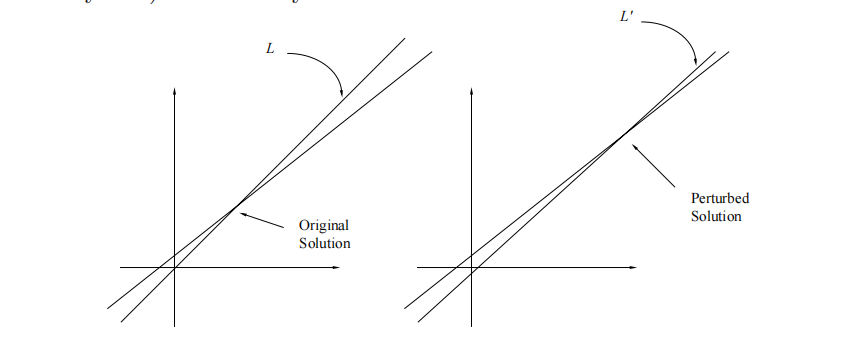
\includegraphics[width=0.8\textwidth]{images/fig1.6.1.png}
    \caption{1.6.1}
    \label{figure1.6.1}
\end{figure}

这在图\ref{figure1.6.1}中得到了说明,其中线 $L$ 被稍微扰动成为线 $L^{\prime}$ 。请注意这个小扰动如何导致交点发生较大变化。这正是例\ref{example1.6.1}中给出的系统的情况。一般来说,病态系统是那些代表几乎平行线、几乎平行平面以及这些概念的概括的系统。

因为舍入误差可以被视为对系统原始系数的扰动,所以即使在病态系统上使用一般良好的数值技术(缺乏精确的算术)也会带来产生无意义结果的风险。

在处理病态系统时,工程师或科学家经常面临比简单地尝试解决系统更基本(有时更令人不安)的问题。即使可以创造一个小奇迹,从而提取出精确的解决方案,科学家或工程师仍然可能得到一个无意义的解决方案,从而导致完全错误的结论。问题源于这样一个事实,即系数通常是凭经验获得的,因此只能在一定的公差范围内得知。对于病态系统,任何系数的微小不确定性都可能意味着解中可能存在极大的不确定性。这种巨大的不确定性甚至可能使精确的解决方案变得毫无用处。

\begin{example}
\label{example1.6.2}
假设方程组:
$$
\begin{cases} 
.835x + .667y = b_1, \\
.333x + .266y = b_2
\end{cases}
$$
中的$b_1$和$b_2$是实验结果,必须从测试仪器的刻度盘上读取。假设刻度盘的读数误差范围为$\pm .001$,且$b_1$和$b_2$的读数分别为$.168$和$.067$,这就构成了示例\ref{example1.6.1}中的病态方程组,并且已知该方程组的精确解为:
\begin{equation}
    (x,y) = (1,-1) \label{equation1.6.1}
\end{equation}
然而,由于刻度盘读数的微小不确定性,我们有:
\begin{equation}
.167 \leq b_1 \leq .169, \quad .066 \leq b_2 \leq .068 \label{equation1.6.2}    
\end{equation}
例如,这意味着读数$(b_1, b_2) = (.168, .067)$对应的解与读数$(b_1, b_2) = (.167, .068)$、$(b_1, b_2) = (.169, .066)$或落在范围(1.6.2)内的任何其他读数对应的解一样有效。对于读数$(b_1, b_2) = (.167, .068)$,精确解为:
\begin{equation}
    (x,y) = (934, -1169) \label{equation1.6.3}
\end{equation}
而对于另一个读数$(b_1, b_2) = (.169, .066)$,精确解为:
\begin{equation}
    (x,y) = (-932, 1167) \label{equation1.6.4}
\end{equation}

你愿意成为第一个乘坐设计中包含该问题解的飞机,或驾驶通过该问题解设计的桥梁的人吗?我不愿意!不确定性太大了。由于解\ref{equation1.6.1}、\ref{equation1.6.3}和\ref{equation1.6.4}中的任何一个都不比其他解更优,因此技术人员如何读取刻度盘上最后一位有效数字,可能会导致采用完全不同的设计方案。由于相关线性方程组的病态性质,飞机或桥梁的成功设计可能取决于运气,而非科学原理。
\end{example}

与其试图从病态方程组中提取精确解,工程师和科学家通常最好将时间和资源投入到重新设计相关实验或数据收集方法上,以避免产生病态方程组。

病态方程组还有另一个令人不安的方面,涉及学生所谓的“检验答案”——将计算出的解代入原方程组的左侧,看它与右侧的接近程度,从而判断解的正确性。更正式地说,若:

$$
x_c = \left(\begin{array}{llll} 
\xi_1 & \xi_2 & \cdots & \xi_n
\end{array}\right)
$$
是方程组:
$$
\begin{cases} 
a_{11}x_1 + a_{12}x_2 + \cdots + a_{1n}x_n = b_1, \\
a_{21}x_1 + a_{22}x_2 + \cdots + a_{2n}x_n = b_2, \\
\vdots \\
a_{n1}x_1 + a_{n2}x_2 + \cdots + a_{nn}x_n = b_n
\end{cases}
$$
的计算解,则称:
$$
r_i = a_{i1}\xi_1 + a_{i2}\xi_2 + \cdots + a_{in}\xi_n - b_i \quad (i = 1, 2, \cdots, n)
$$
为\textbf{残差}。假设你计算出一个解$x_c$,将其代入原方程组后发现所有残差都相对较小,这是否能保证$x_c$接近精确解?令人惊讶的是,当方程组是病态时,答案绝对是否定的!

\begin{example}
\label{example1.6.3}
对于示例\ref{example1.6.3}中的病态方程组,假设你计算出的解为
$$\xi_1 = -666, \quad \xi_2 = 834$$
若你试图通过将其代入原方程组来“检验误差”,使用精确算术计算可得残差:
$$
r_1 = .835\xi_1 + .667\xi_2 - .168 = 0
$$
$$
r_2 = .333\xi_1 + .266\xi_2 - .067 = -.001
$$
也就是说,计算解$(-666, 834)$精确满足第一个方程,且非常接近满足第二个方程。表面上看,这似乎表明计算解应该非常接近精确解。实际上,一个外行甚至可能被误导,认为计算解与精确解的误差在$\pm .001$范围内。显然,事实远非如此,因为精确解是
$$
x = 1, \quad y = -1
$$
对于第一次看到这种情况的学生来说,这总是一个冲击,因为它与新手的直觉相悖。不幸的是,许多学生毕业时仍然认为,通过将计算结果代入原方程,总能“检验”计算的准确性——很高兴你不属于这类学生。
\end{example}

这就引出了一个问题:“如何检验计算解的准确性?”幸运的是,若方程组是良态的,残差确实能更有效地衡量准确性。但这意味着你必须能够回答一些额外的问题,例如:如何预先判断给定的方程组是否是病态的?如何衡量线性方程组的病态程度?

一种确定病态程度的技术可能是:轻微扰动选定的系数,观察解的变化情况。若对某些系数的微小扰动导致解发生显著变化,则说明遇到了病态情况;若某个扰动未导致解发生较大变化,则无法得出结论——可能扰动的是错误的系数集。

通过对不同的系数集进行多次这样的实验,可以对病态程度有一个大致的了解(但不能保证准确)。这种方法成本高昂,且不太令人满意。但在开发出更复杂的工具之前,无法进一步深入讨论。

\begin{exercise}
\label{exercise1.6.1}
考虑示例\ref{example1.6.1}中的病态方程组:
$$
\begin{cases} 
.835x + .667y = .168, \\
.333x + .266y = .067
\end{cases}
$$
\begin{enumerate}[label=(\alph*)]
    \item 描述使用5位算术且不进行尺度变换时,求解该方程组的结果。\label{item1.6.1.a}
    \item 再次使用5位算术,但先对方程组进行行尺度变换,然后再尝试求解,描述这种方法的帮助程度。\label{item1.6.1.b}
    \item 现在使用6位算术且不进行尺度变换,求解该方程组,将结果与精确解进行比较。\label{item1.6.1.c}
    \item 使用6位算术,计算\ref{item1.6.1.c}中解的残差,并解释结果。\label{item1.6.1.d}
    \item 对于(c)中得到的同一个解,此次使用7位算术计算残差,并解释结果。\label{item1.6.1.e}
    \item 总结\ref{item1.6.1.a}到\ref{item1.6.1.e}中的要点,形成结论性陈述。
\end{enumerate}
\end{exercise}

\begin{exercise}
对上述练习\ref{exercise1.6.1}中的病态方程组进行扰动,形成以下方程组:
$$
\begin{cases} 
.835x + .667y = .166995, \\
.333x + .266y = .066995
\end{cases}
$$ 
\begin{enumerate}[label=(\alph*)]
    \item 确定该方程组的精确解,并将其与练习\ref{exercise1.6.1}中方程组的精确解进行比较。\label{item1.6.2.a}
    \item 根据\ref{item1.6.2.a}的结果,就病态方程组的解是否必然会因原方程组的每次扰动而发生显著变化这一问题,形成陈述。
\end{enumerate}
\end{exercise}

\begin{exercise}
考虑由以下两个方程的图像确定的两条直线:
$$
\begin{cases} 
.835x + .667y = .168, \\
.333x + .266y = .067
\end{cases}
$$
\begin{enumerate}[label=(\alph*)]
    \item 使用5位算术计算每条直线的斜率,然后使用6位算术重复计算,在每种情况下,在坐标系中绘制图像。
    \item 通过图形说明,为什么对其中任何一条直线的微小扰动都可能导致解发生较大变化。
    \item 用几何术语描述方程组为最优良态时必须满足的条件。
\end{enumerate}
\end{exercise}

\end{document}
